\documentclass[11pt]{article}
\usepackage[margin=1.02in]{geometry}
\usepackage{amsmath,amssymb,amsthm,mathtools}
\usepackage{array,booktabs,longtable,tabularx}
\usepackage{enumitem,microtype,xcolor}
\usepackage{tikz}
\usetikzlibrary{arrows.meta,positioning,backgrounds}
\usepackage[colorlinks=true,linkcolor=blue!55!black,urlcolor=blue!55!black]{hyperref}

\newtheorem{theorem}{Theorem}[section]
\newtheorem{lemma}[theorem]{Lemma}
\theoremstyle{definition}
\newtheorem{definition}[theorem]{Definition}
\newtheorem{remark}[theorem]{Remark}
\newcommand{\N}{\mathbb N}
\newcommand{\Pow}{\mathcal P}
\newcommand{\State}{\Sigma}
\newcommand{\Event}{\mathsf{Event}}
\newcommand{\Replica}{\mathsf{Replica}}
\newcommand{\Version}{\mathsf{Version}}
\newcommand{\Time}{\mathsf{Timestamp}}
\newcommand{\init}{\sigma_0}
\newcommand{\applySeq}{\mathsf{applySeq}}
\newcommand{\doop}{\mathsf{do}}
\newcommand{\merge}{\mathsf{merge}}
\newcommand{\query}{\mathsf{query}}
\newcommand{\vis}{\mathrel{\mathsf{vis}}}
\newcommand{\rc}{\mathrel{\xrightarrow{\mathsf{rc}}}}
\newcommand{\loOn}{\mathsf{loOn}}
\newcommand{\lo}{\mathsf{lo}}
\newcommand{\Can}{\mathsf{Canonical}}
\newcommand{\reach}{\mathrel{\mathsf{Reaches}}}
\newcommand{\none}{\bot}
\newcommand{\lean}[1]{\texttt{#1}}
\newcommand{\src}[2]{\href{../../#1}{\texttt{#2}}}
\newcommand{\anchor}[2]{\par\smallskip\noindent\emph{Lean: }\src{#1}{#2}.}
\newenvironment{semanticrule}[1]
  {\par\medskip\noindent
   \begin{minipage}[t]{0.13\textwidth}\raggedright\scshape #1\end{minipage}%
   \begin{minipage}[t]{0.84\textwidth}\centering\vspace{-1ex}}
  {\end{minipage}\par\medskip}
\tikzset{
  layer/.style={rectangle,rounded corners,draw=blue!55!black,
    fill=blue!3,align=center,inner sep=5pt},
  result/.style={rectangle,rounded corners,draw=orange!70!black,
    fill=orange!4,align=center,inner sep=5pt},
  flow/.style={-{Latex[length=2mm]},semithick}}
\setlist{nosep,leftmargin=*}
\setlength{\emergencystretch}{2em}
\sloppy
\title{Formal Semantics and Theorem Reference\\
  for Mergeable Replicated Data Types}
\author{Anonymous Authors}
\date{}
\hypersetup{pdftitle={Formal Semantics and Theorem Reference for MRDTs},
  pdfauthor={Anonymous Authors},bookmarksopen=true,bookmarksnumbered=true}

\begin{document}
\maketitle

\begin{abstract}
This document gives a bottom-up reference for the public formal theory of
mergeable replicated data types (MRDTs) mechanized in Lean~4. It starts with
events and datatype signatures, defines the version-DAG operational semantics,
then explains how finite event histories determine stored states, which merge
property preserves that explanation, and how operation-generation constraints
connect it to an independent client specification. It also covers merge-base
construction for version DAGs without a single greatest common ancestor and
two independent garbage-collection refinements. Definitions are ordered by
semantic dependence rather than Lean file order. Every principal definition
and theorem has its exact Lean declaration and a source link. Proof-local
lemmas are omitted from the main line; the historical binary development is
isolated in an appendix.
\end{abstract}

\tableofcontents

\section{Purpose and evidence boundary}

This document is written for readers who want to understand the formal theory
before navigating its Lean implementation.  It reconstructs the interface and
theorem dependency graph and then instantiates them for every released RDT. It
answers four questions:
\begin{enumerate}
\item What are the exact states and transitions of the MRDT machine?
\item What invariant makes every stored version replayable, and what
  obligation preserves it at merge?
\item How is internal replay connected to an independent client specification?
\item Which history- and state-collection steps refine the same uncollected
  semantics?
\end{enumerate}

The top-level result is client-facing: every released datatype packages an
issuance discipline, a merge-adequacy proof, an independent sequential
specification, and a refinement proof. Consequently, every version produced
by an issuance-certified ordinary or virtual-merge-base execution admits a
legal sequential history with the same events and the same query results.
Sections~2--8 define the layers needed by this statement.
Sections~\ref{sec:history-gc}--\ref{sec:state-gc} add optional history-
and datatype-state collection refinements. Section~\ref{sec:instances}
then presents the complete datatype packages and their collection status.

\paragraph{Reader's map.}
\renewcommand{\arraystretch}{1.08}
\begin{longtable}{@{}>{\raggedright\arraybackslash}p{0.20\textwidth}
  >{\raggedright\arraybackslash}p{0.58\textwidth}
  >{\raggedright\arraybackslash}p{0.12\textwidth}@{}}
\toprule
Layer & Contract and consequence & Location\\
\midrule
\endhead
Operational machine & Events and the datatype signature determine fork,
apply, query, and ternary merge in a version DAG. & Sections~2--3\\
Replay model & A finite event set admits a respecting replay under the
sufficient replay laws, which also make its fold unique. & Sections~4--5\\
Merge preservation & An all-context or restricted merge theorem preserves
a canonical state at a merge step. Execution invariants provide another
proof route. & Section~6\\
Client correctness & Issuance, one visibility-plus-$rc$ order, an independent
sequential machine, and a representation relation turn internal replay into
observable sequential correctness. & Section~7\\
Virtual bases & A recursive fold over maximal common ancestors constructs the
canonical intersection state when no stored GCA exists. & Section~8\\
Released instances & Each package records its representation, issuance
policy, merge theorem, sequential specification, relation, and proof route. &
Section~\ref{sec:instances}\\
Collection & Commit-history and datatype-state collection refine the same
uncollected semantics and compose by trace erasure; the datatype profiles
state what each released representation can presently reclaim. &
Sections~\ref{sec:history-gc}--\ref{sec:state-gc}\\
\bottomrule
\end{longtable}
\renewcommand{\arraystretch}{1}

The mathematical displays are transcriptions or notation-level expansions of
the cited declarations. The trusted computing base for machine-checked
statements is Lean's kernel and the axioms reported by the ledger; Mathlib
supplies checked library proofs. The transcription, notation, prose,
and links remain review obligations. No claim is made that a separately
implemented runtime is extracted from Lean.

\begin{figure}[ht]
\centering
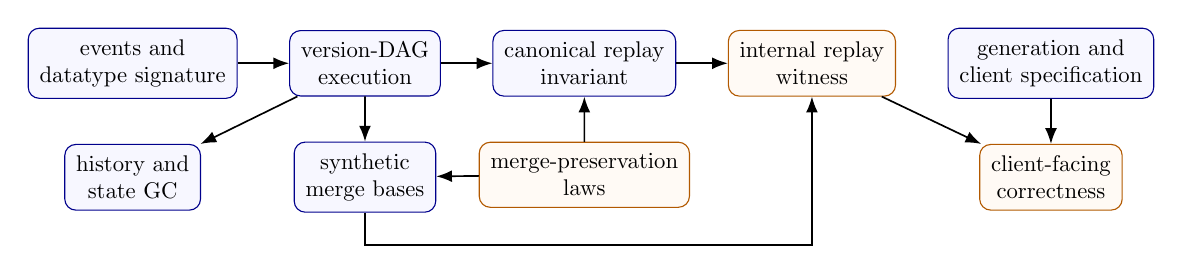
\begin{tikzpicture}[scale=.82,transform shape,node distance=7mm and 8mm]
  \node[layer] (sig) {events and\\datatype signature};
  \node[layer,right=of sig] (exec) {version-DAG\\execution};
  \node[layer,right=of exec] (canon) {canonical replay\\invariant};
  \node[result,below=of canon] (join) {merge-preservation\\laws};
  \node[result,right=of canon] (replay) {internal replay\\witness};
  \node[layer,right=of replay] (client) {generation and\\client specification};
  \node[result,below=of client] (correct) {client-facing\\correctness};
  \node[layer,below=of exec] (vbase) {synthetic\\merge bases};
  \node[layer,below=of sig] (gc) {history and\\state GC};
  \draw[flow] (sig)--(exec);
  \draw[flow] (exec)--(canon);
  \draw[flow] (join)--(canon);
  \draw[flow] (canon)--(replay);
  \draw[flow] (replay)--(correct);
  \draw[flow] (client)--(correct);
  \draw[flow] (exec)--(vbase);
  \draw[flow] (join)--(vbase);
  \draw[flow] (vbase.south) -- ++(0,-5mm) -| (replay.south);
  \draw[flow] (exec)--(gc);
\end{tikzpicture}
\caption{Semantic dependency order. Arrows point from prerequisite to
consumer. The two GC layers are optional refinements, not premises of
client-facing correctness.}
\label{fig:dependency}
\end{figure}

\section{Primitive types and datatype signatures}

\subsection{Identifiers and events}

Replicas, timestamps, and versions are natural numbers:
\[
  \Replica=\N,\qquad \Time=\N,\qquad \Version=\N.
\]
For an application-operation type $O$, an event is
\[
  \Event(O)=\Time\times\Replica\times O.
\]
If $e=(t,r,o)$, write $\mathsf{time}(e)=t$ and
$\mathsf{rep}(e)=r$. Timestamps are Lamport
timestamps. Global uniqueness and causal monotonicity are properties of valid
configurations and the apply transition, not of the bare product type.
\anchor{Sal/MRDTs/Framework/Base/UpdateSignature.lean}
  {Foundation.Replica, Foundation.Timestamp, Foundation.Op}

\begin{definition}[MRDT signature]
An MRDT signature is
\[
 D=(\State,\init,O,Q,R,\doop,\merge,\query)
\]
with decidable equality on $\State$ and $O$, and
\[
\begin{aligned}
 \doop&:\State\to\Event(O)\to\State,\\
 \merge&:\State\to\State\to\State\to\State,\\
 \query&:\State\to Q\to R.
\end{aligned}
\]
The intended reading of $\merge(l,a,b)$ is a three-way merge with ancestor
state $l$ and branch states $a,b$.
The ancestor is semantically necessary for datatypes whose state combines by
addition rather than idempotent union: the flat counter, for example, uses
$\merge(l,a,b)=a+b-l$ so that effects already present in both branches are
counted once.  Ternary merge covers both these group-like states and ordinary
grow-only unions with one interface.
The paper's $\doop$ is the Lean field \lean{MRDTSig.update}; Lean reserves
\lean{do} for its term syntax.
\anchor{Sal/MRDTs/Framework/Signature.lean}{MRDTSig}
\end{definition}

This signature is the semantic datatype interface; some models use
noncomputable queries. Verification attaches
replay, merge, generation, and client certificates to this same $D$.

\paragraph{Running example: RGA.}
The production RGA stores grow-only insertion and deletion facts:
\[
\begin{aligned}
 \State_{\mathrm{RGA}}
   &=(\N^2\to\mathsf{Bool})\times(\N\to\mathsf{Bool}),\\
 O_{\mathrm{RGA}}&=\mathsf{addAfter}(\mathit{anchor})
                 \mid\mathsf{remove}(\mathit{id}).
\end{aligned}
\]
An insertion's timestamp is its identifier. The event sets the birth bit
indexed by that identifier and its anchor; a removal sets the tombstone bit
for its identifier. Merge is
pointwise Boolean union of the GCA and two branch states. The query sorts the
finite insertion support, inserts each identifier after its anchor, and
filters tombstoned identifiers. Thus the implementation state is unordered
grow-only evidence, while the client observes an ordinary list.
\anchor{Sal/MRDTs/Instances/RGA.lean}{RGA.RGAM, RGA.rgaUpdate, RGA.read}

\subsection{Finite replay}

Finite replay uses only the merge-free projection
\[
 D_U=(\State,\init,O,\doop).
\]
Lean calls this derived structure \lean{UpdateSig}; it retains precisely the
fields used when an event history is folded.

For $\pi=[e_1,\ldots,e_n]$,
\[
 \applySeq(D,s,\pi)
   =\doop(\cdots\doop(\doop(s,e_1),e_2)\cdots,e_n).
\]
A list enumerates a set exactly when
\[
 \mathsf{listPermOf}(\pi,E)
 \Longleftrightarrow
 \mathsf{Nodup}(\pi)\land \forall e.\;(e\in\pi\leftrightarrow e\in E).
\]
It respects a relation $R$ when no later element is required to precede an
earlier one:
\[
 \mathsf{respects}(\pi,R)
 \Longleftrightarrow
 \mathsf{Pairwise}_{\pi}(\lambda a\ b.\;\neg R(b,a)).
\]
\anchor{Sal/MRDTs/Framework/Base/Replay.lean}
  {Foundation.applySeq, Foundation.listPermOf, Foundation.respects}

Concrete updates commute when applying them in either order gives the same
implementation state, from every starting state:
\[
 e_1\leftrightarrow e_2
 \Longleftrightarrow
 \forall s:\State.\;
 \doop(\doop(s,e_1),e_2)=\doop(\doop(s,e_2),e_1).
\]

A replay policy $P$ determines a directed relation on events, written
$e_1\rc e_2$: replay $e_1$ before $e_2$ to resolve their conflict.
Lean represents the policy by a resolver with results
\lean{Fst\_then\_snd}, \lean{Snd\_then\_fst}, and \lean{Either};
the directed relation is precisely \lean{ReplayPolicy.Before}, which tests
for \lean{Fst\_then\_snd}. The theory tests the reverse edge on the reversed
pair. The carrier alone does not guarantee that a \lean{Snd\_then\_fst}
verdict agrees with that reverse test.
The relation specifies the intended resolution of concurrent events; it is
not defined by concrete-update noncommutation. For example, LWW resolves
concurrent writes by increasing timestamp, although its concrete updates
retain the maximum timestamp and commute. The default policy returns
$\mathsf{Either}$. Each public package selects one such policy. The sequential
legality predicate may impose additional constraints on the witness list;
these must also be stated in the datatype's contract.
Section~\ref{sec:rc-order} derives its set-relative client relation once
replay contexts have supplied visibility and the finite event set. Finite
replay, commutation, and the policy are factored through the merge-free
projection of $D$.
\anchor{Sal/MRDTs/Framework/Base/UpdateSignature.lean}
  {Foundation.UpdateSig.commutes, Foundation.RcRes,
   Foundation.ReplayPolicy, Foundation.ReplayPolicy.Before,
   Foundation.UpdateSig.rc}
\anchor{Sal/MRDTs/Metatheory/ProductionLedger.lean}{Production.registry}

\section{Version-DAG operational semantics}
\label{sec:execution}

\subsection{Graph order}

For $P:\Version\to\mathsf{List}(\Version)$,
\[
 \mathsf{Reaches}(P,a,b)
 \Longleftrightarrow
 (\lambda x\ y.\;x\in P(y))^*(a,b).
\]
The ordinary merge rule uses a greatest-common-ancestor predicate:
\[
\begin{aligned}
 \mathsf{IsGCA}(P,v_1,v_2,v_T)\Longleftrightarrow{}&
 v_T\reach v_1\land v_T\reach v_2\\
 &\land\forall w.\;w\reach v_1\to w\reach v_2\to w\reach v_T.
\end{aligned}
\]
Every common ancestor reaches a GCA. Ranked reachability is antisymmetric, so
a GCA is unique when it exists. A criss-cross DAG may instead have several
incomparable maximal common ancestors and no GCA; Section~8 constructs its
virtual merge base.
\anchor{Sal/MRDTs/Framework/Execution.lean}{Reaches, IsGCA}
\anchor{Sal/MRDTs/Metatheory/StoreInvariant.lean}{isGCA\_unique}

For a pair of versions $a,b$, define
\[
\begin{aligned}
 \mathsf{CommonAncestors}(P,a,b)&=
 \{x\mid x\reach a\land x\reach b\},\\
 \mathsf{IsMaximalCommonAncestor}(P,a,b,m)&\Longleftrightarrow
 m\in\mathsf{CommonAncestors}(P,a,b)\\
 &\quad\land\forall x\in\mathsf{CommonAncestors}(P,a,b).\;
   m\reach x\to x=m.
\end{aligned}
\]
Thus $m$ is maximal when no distinct common ancestor descends from it. The
self-case is present because $\mathsf{Reaches}$ is reflexive. Several
incomparable versions may satisfy this predicate.
\anchor{Sal/MRDTs/Framework/Execution.lean}
  {CommonAncestors, IsMaximalCommonAncestor}

\subsection{Configurations}

For an MRDT $D$, write the version store as a partial map and let
$A_C=\mathsf{dom}(S)$ be its allocated-version set. A configuration contains
\[
\begin{array}{rcl@{\qquad}l}
 S&:&\Version\rightharpoonup(\State\times\Pow(\Event(O)))
   &\text{allocated version contents},\\
 H&:&\Replica\rightharpoonup A_C&\text{active replica heads},\\
 P&:&\Version\to\mathsf{List}(\Version)&\text{parent lists},\\
 \vis&:&\Event(O)\to\Event(O)\to\mathsf{Prop}&\text{visibility}.
\end{array}
\]
Thus $C=\langle S,H,P,\vis\rangle$. Write
\[
\begin{aligned}
 \mathsf{state}_C&:A_C\to\State,&
 \mathsf{state}_C(v)&=\mathsf{fst}(S(v)),\\
 \mathsf{events}_C&:A_C\to\Pow(\Event(O)),&
 \mathsf{events}_C(v)&=\mathsf{snd}(S(v)),\\
 \mathsf{headState}_C&=\mathsf{state}_C\circ H,&
 \mathsf{headEvents}_C&=\mathsf{events}_C\circ H.
\end{aligned}
\]
The configuration's active event universe is
\[
\begin{aligned}
 C.\mathsf{events}&\equiv
 \{e\mid\exists r,E.\;
   \mathsf{headEvents}_C(r)=E\land e\in E\}\\
 &=\bigcup_{r\in\mathsf{dom}(H)}\mathsf{headEvents}_C(r).
\end{aligned}
\]
It contains the events observed at active replica heads, not the union of all
historical version event sets. These functions and the active event universe
are derived observations, not configuration components.
\anchor{Sal/MRDTs/Framework/Execution.lean}{Configuration.events}

For any partial map $f$, write
$f(x)=\none\Longleftrightarrow x\notin\mathsf{dom}(f)$.

A well-formed semantic configuration satisfies:
\begin{enumerate}
\item Every visibility endpoint occurs in some $\mathsf{headEvents}_C(r)$,
  and each head event set is closed under visibility.
\item Distinct active events have distinct timestamps;
  $e_1\vis e_2$ implies $\mathsf{time}(e_1)<\mathsf{time}(e_2)$; and distinct
  events from one replica are visibility-comparable.
\item Parents have smaller version numbers and $S(0)=(\init,\varnothing)$.
\item If $S(v_i)=(s_i,E_i)$ for $i\in\{1,2,T\}$ and $v_T$ is a GCA of
  $v_1,v_2$, then $E_T=E_1\cap E_2$.
\end{enumerate}
Thus a configuration is already an operationally well-formed state. Client
safety and canonical replay are separate predicates.
\anchor{Sal/MRDTs/Framework/Execution.lean}{Configuration}

Lean totalizes the two partial maps: \lean{ver} and \lean{head} return
\lean{Option}, while \lean{parents} is the total function $P$. The
\lean{head\_alloc} field implements the paper type $H:\Replica\rightharpoonup
A_C$. The functions \lean{Configuration.headState} and
\lean{Configuration.headEvents} implement the two partial compositions above.
The store invariant in Section~3.4 connects $P$ to $A_C$: every version named
in a parent list must lie in $A_C$. Until that invariant is imposed, keeping
$P$ total avoids adding a second allocation domain.

Write $\mathsf{initConfig}(D)$ for the initial configuration. It has replica
$0$ at version $0$, both with state $\init$ and empty event set. All other
replicas and versions are absent, parent lists are empty, and visibility is
empty.
\anchor{Sal/MRDTs/Framework/Execution.lean}{initConfig}

\subsection{Labels, freshness, and transition rules}

The label constructors have explicit types
\[
\begin{array}{rcl}
 \mathsf{fork}&:&\Replica\to\Replica\to\mathsf{Label}(D),\\
 \mathsf{apply}&:&\Time\to\Replica\to O\to\mathsf{Label}(D),\\
 \mathsf{merge}&:&\Replica\to\Replica\to\mathsf{Label}(D),\\
 \mathsf{query}&:&\Replica\to Q\to R\to\mathsf{Label}(D).
\end{array}
\]
Fork is destination-first: $\mathsf{fork}(r_d,r_s)$.
\anchor{Sal/MRDTs/Framework/Execution.lean}{Label}

Write $\mathsf{freshTime}(C,t)$ when no event at an allocated version has
timestamp $t$, and $\mathsf{freshVer}(C,v')$ when $v'\notin A_C$.
The condition $v<v'$ is a rank condition for the version DAG, not a timestamp
comparison. It makes the parent relation well founded. The following rules
display all changed semantic fields; other entries remain unchanged, and the
resulting configuration satisfies the configuration conditions above.

\begin{semanticrule}{Fork}
\[
\frac{
 \begin{gathered}
 H(r_s)=v\quad \mathsf{headState}_C(r_s)=s\quad
 \mathsf{headEvents}_C(r_s)=E\\
 H(r_d)=\none\quad \mathsf{freshVer}(C,v')\quad v<v'
 \end{gathered}
}{
 C\xrightarrow{\mathsf{fork}(r_d,r_s)}
 C\!\left[\begin{aligned}
 S(v')&\mapsto(s,E),&H(r_d)&\mapsto v',&P(v')&\mapsto[v]
 \end{aligned}\right]}
\]
\end{semanticrule}
Fork creates a fresh child of an existing source head, preserving that source
as the child's parent.
\anchor{Sal/MRDTs/Framework/Execution.lean}{Step.fork}
\anchor{Sal/MRDTs/Framework/Execution.lean}
  {Step.fork\_copies\_source, Step.fork\_head\_ne\_root}

\begin{semanticrule}{Apply}
\[
\frac{
 \begin{gathered}
 H(r)=v\quad \mathsf{headState}_C(r)=s\quad
 \mathsf{headEvents}_C(r)=E\quad e=(t,r,o)\\
 \mathsf{freshTime}(C,t)\quad \mathsf{freshVer}(C,v')\quad v<v'
 \end{gathered}
}{
 C\xrightarrow{\mathsf{apply}(t,r,o)}
 C\!\left[\begin{aligned}
 S(v')&\mapsto(\doop(s,e),E\cup\{e\}),&H(r)&\mapsto v',\\
 P(v')&\mapsto[v],&\vis&\mapsto\vis\cup(E\times\{e\})
 \end{aligned}\right]}
\]
\end{semanticrule}
Freshness gives globally unique timestamps. Because the resulting configuration
also satisfies causal timestamp monotonicity, all events visible to $e$ have
smaller timestamps.
Together these are the Lamport-clock conditions. The raw rule has no issuance
premise.
\anchor{Sal/MRDTs/Framework/Execution.lean}{Step.apply}

\begin{semanticrule}{Query}
\[
\frac{\mathsf{headState}_C(r)=s\qquad z=\query(s,q)}
 {C\xrightarrow{\mathsf{query}(r,q,z)}C}
\]
\end{semanticrule}
Query is observational.
\anchor{Sal/MRDTs/Framework/Execution.lean}{Step.query}

\begin{semanticrule}{Merge}
\[
\frac{
 \begin{gathered}
 H(r_i)=v_i\quad \mathsf{headState}_C(r_i)=s_i\quad
 \mathsf{headEvents}_C(r_i)=E_i\qquad(i\in\{1,2\})\\
 \mathsf{IsGCA}(P,v_1,v_2,v_T)\quad
 \mathsf{state}_C(v_T)=s_T\quad \mathsf{events}_C(v_T)=E_T\\
 \mathsf{freshVer}(C,v_m)\quad v_1<v_m\quad v_2<v_m
 \end{gathered}
}{
 C\xrightarrow{\mathsf{merge}(r_1,r_2)}
 C\!\left[\begin{aligned}
 S(v_m)&\mapsto(\merge(s_T,s_1,s_2),E_1\cup E_2),\\
 H(r_1)&\mapsto v_m,&P(v_m)&\mapsto[v_1,v_2]
 \end{aligned}\right]}
\]
\end{semanticrule}
The first replica receives the merged head. Merge creates no event.
\anchor{Sal/MRDTs/Framework/Execution.lean}{Step.merge}

\subsection{Store invariant and GCA events}

The store invariant has three components. First, define
\[
\mathsf{ParentsAllocated}(S,P)\Longleftrightarrow
 \forall v,p.\;p\in P(v)\Rightarrow p\in\mathsf{dom}(S).
\]
Every parent named by an edge is present in the version store.
Under this condition, $P$ may be viewed as
$P:\Version\to\mathsf{List}(A_C)$, and its restriction to allocated children
has type $P|_{A_C}:A_C\to\mathsf{List}(A_C)$.
Define event monotonicity along a parent edge by
\[
\begin{aligned}
\mathsf{EventsMonotone}(S,P)\Longleftrightarrow
 \forall v,p,s_p,E_p,s_v,E_v.\;&
 p\in P(v)\land S(p)=(s_p,E_p)\land S(v)=(s_v,E_v)\\
 &\Rightarrow E_p\subseteq E_v.
\end{aligned}
\]
Thus a child contains every event stored at its parent. Finally, define
\[
\begin{aligned}
\mathsf{EventOrigin}(S,P)\Longleftrightarrow
 \forall v,s,E,e.\;&S(v)=(s,E)\land e\in E\Rightarrow\\
 &\exists v_0,s_0,E_0.\;S(v_0)=(s_0,E_0)\land e\in E_0\\
 &\quad\land\forall w,s_w,E_w.\;
 S(w)=(s_w,E_w)\land e\in E_w\\
 &\hspace{11em}\Rightarrow\mathsf{Reaches}(P,v_0,w).
\end{aligned}
\]
Every stored event therefore has an allocated origin version containing it;
that version is an ancestor of every allocated version containing the event.
No uniqueness of the origin is asserted. The store invariant is the conjunction
\[
\begin{aligned}
\mathsf{StoreInv}(S,P)\Longleftrightarrow{}&
 \mathsf{ParentsAllocated}(S,P)\\
 &\land\mathsf{EventsMonotone}(S,P)\\
 &\land\mathsf{EventOrigin}(S,P).
\end{aligned}
\]
These three predicates correspond respectively to Lean's
\lean{parents\_alloc}, \lean{events\_mono}, and \lean{origin} fields.
The proof of the GCA event equation factors through their conjunction. Its
principal consequence is
\[
\begin{gathered}
 \mathsf{StoreInv}(S,P)\land\mathsf{IsGCA}(P,v_1,v_2,v_T)\\
 \land S(v_i)=(s_i,E_i)\;(i\in\{1,2,T\})
 \Longrightarrow E_T=E_1\cap E_2.
\end{gathered}
\]
\anchor{Sal/MRDTs/Metatheory/StoreInvariant.lean}
  {StoreInv, gca\_events\_of\_storeInv}

\section{Replay contexts and set-relative order}
\label{sec:replay}

\subsection{Replay context}

For a stored event set $E$, the replay problem is to enumerate exactly the
events in $E$ in an admissible order and fold their updates from $\init$.
Admissibility depends on which events have been observed and on their
visibility relation. It does not depend on version identifiers, parent edges,
materialized states, or merge bases. The replay context isolates this smaller
input to the ordering proofs.

Let $L:\Replica\rightharpoonup\Pow(\Event(O))$ map each active replica to the
event set at its current head. Here $a\vis b$ means that $a$ is visible to
$b$, so $a$ causally precedes $b$. Define the observed event universe by
\[
 \mathsf{Observed}_L(e)\Longleftrightarrow
 \exists r,E.\;L(r)=E\land e\in E.
\]
The two required coherence conditions are
\[
\begin{aligned}
 \mathsf{TimestampUnique}(L)\Longleftrightarrow{}&
 \forall a,b.\;\mathsf{Observed}_L(a)\land\mathsf{Observed}_L(b)\land a\ne b
 \Rightarrow \mathsf{time}(a)\ne\mathsf{time}(b),\\
 \mathsf{SameReplicaTotal}(L,\vis)\Longleftrightarrow{}&
 \forall a,b.\;\mathsf{Observed}_L(a)\land\mathsf{Observed}_L(b)\land a\ne b\\
 &\hspace{5em}\land\mathsf{rep}(a)=\mathsf{rep}(b)
 \Rightarrow a\vis b\lor b\vis a.
\end{aligned}
\]
Thus timestamps identify observed events globally, while visibility compares
every pair of distinct events issued by one replica. A replay context is
formally
\[
 \mathsf{ReplayContext}(D)=
 \left\langle
 \begin{array}{l}
 L:\Replica\rightharpoonup\Pow(\Event(O)),\\
 \vis:\Event(O)\to\Event(O)\to\mathsf{Prop},\\
 u_{\mathrm{ts}}:\mathsf{TimestampUnique}(L),\\
 u_{\mathrm{rep}}:\mathsf{SameReplicaTotal}(L,\vis)
 \end{array}
 \right\rangle .
\]
For a replay context $R=\langle L,\vis,u_{\mathrm{ts}},u_{\mathrm{rep}}\rangle$,
the event universe is the union of the active replicas' head-event sets:
\[
 R.\mathsf{events}
 =\{e\mid\mathsf{Observed}_L(e)\}
 =\bigcup_{r\in\mathsf{dom}(L)}L(r).
\]
Every MRDT configuration $C$ projects to a replay context by taking
$L=\mathsf{headEvents}_C$ and retaining $C.\vis$. The configuration fields
\lean{timestamps\_distinct} and \lean{vis\_total\_same\_replica} supply the
two proofs. Lean totalizes $L$ as an Option-valued function;
\lean{ReplayContext.L} receives the derived head-event map, and
\lean{Configuration.replayContext} constructs the projection.
Write $R_C=\mathsf{replayContext}(C)$ for this projection whenever $C$ is an
MRDT configuration. The projection preserves the active event universe:
\[
 R_C.\mathsf{events}=C.\mathsf{events}.
\]
\anchor{Sal/MRDTs/Framework/Base/ReplayContext.lean}
  {Foundation.ReplayContext}
\anchor{Sal/MRDTs/Framework/Execution.lean}{Configuration.replayContext}

\subsection{Resolve-conflict relation and set-relative linearization}

Fix a replay policy $P$ and its directed relation $rc$ as defined in Section~2.
The relation expresses the datatype's resolution policy independently
of its implementation. For concurrent LWW writes with distinct timestamps,
\[
 a\rc b\Longleftrightarrow \mathsf{time}(a)<\mathsf{time}(b).
\]
The implementation retains the maximum timestamp regardless of delivery
order; an ordinary overwrite replay places the smaller timestamp first.

\label{sec:rc-order}

The resolve-conflict relation now supplies the directed policy edge used by
linearization. For replay context $R$, version event set $E$, and events
$e_1,e_2$, define the set-relative linearization relation by
\[
\begin{aligned}
 e_1\;\loOn_{R,E}\;e_2\Longleftrightarrow
 &(e_1\vis e_2\land(e_1\rc e_2\lor e_2\rc e_1))\\
 {}\lor{}&(\neg(e_1\vis e_2)\land\neg(e_2\vis e_1)
 \land e_1\rc e_2\\
 &\quad\land\neg\exists e_3\in E.\;
 e_2\vis e_3\land(e_2\rc e_3\lor e_3\rc e_2)).
\end{aligned}
\]
An event $e_3\in E$ satisfying the final existential condition is an
\emph{absorber} for $e_2$. Only an absorber inside $E$ can remove an
arbitration edge needed to replay $E$. Growing the set may add absorbers and
therefore remove such edges:
\[
 E\subseteq E'\land a\;\loOn_{R,E'}\;b\Longrightarrow a\;\loOn_{R,E}\;b.
\]
The historical global order searches for absorbers without the membership
restriction. Every historical edge is an edge of $\loOn_{R,E}$. It agrees
with $\loOn_{R,R.\mathsf{events}}$ when visibility targets belong to
$R.\mathsf{events}$, as they do for a configuration's replay context.
The set parameter is therefore essential in the general theory: whether an
arbitration edge is needed depends on whether its absorber belongs to the
particular version being replayed, not merely on the global event universe.
\anchor{Sal/MRDTs/Metatheory/Join/SetRelativeReplay.lean}
  {Foundation.loOn, Foundation.loOn\_mono, Foundation.loOn\_of\_lo}

For an all-$\mathsf{Either}$ policy, $rc$ has no edges and therefore
\[
 \neg(a\;\loOn_{R,E}\;b).
\]
In particular, $\mathsf{Either}$ does not mean ``retain all visibility.''
Visibility contributes to $\loOn$ only for a pair that $rc$ classifies as a
conflict.

\paragraph{RGA instance.}
RGA insertion and tombstone updates commute at the raw storage layer, but its
ordinary-list specification still has conflicts. Its sole $rc$ relation
orders the RGA conflicts described in Section~\ref{sec:instances}; $\loOn$ uses that relation
directly.
\anchor{Sal/MRDTs/Instances/RGASequential.lean}{RGA.rc}

\subsection{Sufficient replay laws and convergence}

The following optional algebraic laws are one sufficient route to replay
convergence under $P$. They are not the definition of $rc$ and are not
required fields of the public datatype certificate. In this subsection and
the replay theorems below, $D$ and $P$ are fixed together.

Write
\[
 \mathsf{distinct}(a,b)\Longleftrightarrow
 \mathsf{time}(a)\ne\mathsf{time}(b).
\]
Replay contexts make this equivalent to event inequality on observed events.
The update-layer bundle has three conjuncts. Coverage of concrete
noncommuting pairs is
\[
\begin{aligned}
 \mathsf{NoncommCovered}(D,P)\Longleftrightarrow
 \forall a,b.\;&
 \neg(a\leftrightarrow b)\Longrightarrow
 (a\rc b\lor b\rc a).
\end{aligned}
\]
This is a one-way proof obligation: a pair not ordered in either direction
must commute concretely. An ordered pair may also commute. In particular,
all-commuting updates satisfy coverage for every choice of $rc$.
Write $Q^{+}(a,b)$ when there is a nonempty finite $Q$-path from $a$ to $b$,
and define
\[
 \mathsf{Acyclic}(Q)\Longleftrightarrow
 \forall a.\;\neg Q^{+}(a,a).
\]
Resolve-conflict acyclicity is
\[
 \mathsf{RcAcyclic}(D,P)\Longleftrightarrow
 \mathsf{Acyclic}(\lambda a\,b.\;a\rc b).
\]
It permits policy chains of arbitrary finite length and rules out only directed
cycles. Finally,
conditional commutation lift is
\[
\begin{aligned}
 \mathsf{CondCommLift}(D,P)\Longleftrightarrow
 \forall s,e,e',e'',\pi.\;&
 \mathsf{distinct}(e,e')\land\mathsf{distinct}(e,e'')
 \land\mathsf{distinct}(e',e'')\\
 &\land e\rc e'
 \land(e'\rc e''\lor e''\rc e')\\
 &\Longrightarrow
 \doop(\applySeq(D,\doop(\doop(s,e'),e),\pi),e'')\\
 &\qquad=
 \doop(\applySeq(D,\doop(\doop(s,e),e'),\pi),e'').
\end{aligned}
\]
Therefore
\[
 \mathsf{ReplayLaws}(D,P)\Longleftrightarrow
 \mathsf{NoncommCovered}(D,P)\land
 \mathsf{RcAcyclic}(D,P)\land
 \mathsf{CondCommLift}(D,P).
\]
These conjuncts correspond respectively to Lean's
\lean{noncomm\_covered}, \lean{rc\_acyclic}, and
\lean{cond\_comm\_lift} fields.
The conditional swap uses the $rc$-related successor tested by the
linearization relation above; that successor need not be concretely
noncommuting. When all concrete updates commute, both swap orders already
agree before the successor is applied. Thus every acyclic $rc$ satisfies
these sufficient laws for an all-commuting implementation.
\anchor{Sal/MRDTs/Framework/ReplayLaws.lean}
  {RcAcyclic, ReplayLaws, ReplayLaws.of\_all\_comm}

With these laws, transitive and irreflexive visibility, and finite support,
$\loOn_{R,E}$ is acyclic on $E$, admits a respecting enumeration, and all
respecting enumerations fold to the same state. Intuitively, acyclicity says
that the replay constraints are jointly schedulable; existence produces at
least one such schedule; and convergence says that choosing a different valid
schedule cannot change the result. Thus a finite event set $E$ determines one
replayed state even when it admits several valid orders.

For events in $E$, write
\[
 a\;\loOn^{\ne}_{R,E}\;b
 \Longleftrightarrow
 a\ne b\land a\in E\land b\in E\land a\;\loOn_{R,E}\;b.
\]
\begin{lemma}[Existence and uniqueness of set-relative replay]
\label{lem:set-relative-replay}
Suppose
\[
\begin{gathered}
 \mathsf{RcAcyclic}(D,P),\qquad
 \mathsf{Transitive}(R.\mathsf{vis}),\qquad
 \mathsf{Irreflexive}(R.\mathsf{vis}),\\
 E\subseteq R.\mathsf{events},\qquad
 \mathsf{listPermOf}(\ell,E).
\end{gathered}
\]
Then:
\begin{enumerate}
\item $\loOn^{\ne}_{R,E}$ is acyclic:
\[
 \mathsf{Acyclic}
   (\lambda a\,b.\;a\;\loOn^{\ne}_{R,E}\;b).
\]
\item $E$ has a respecting enumeration:
\[
 \exists\rho.\;
 \mathsf{listPermOf}(\rho,E)\land
 \mathsf{respects}(\rho,\loOn_{R,E}).
\]
\item if $\mathsf{ReplayLaws}(D,P)$ also holds, all respecting enumerations
of $E$ have the same fold, from every starting state:
\[
\begin{aligned}
 \forall s,\rho_1,\rho_2.\quad
 &\mathsf{listPermOf}(\rho_1,E)
 \land\mathsf{listPermOf}(\rho_2,E)\\
 &\land\mathsf{respects}(\rho_1,\loOn_{R,E})
 \land\mathsf{respects}(\rho_2,\loOn_{R,E})\\
 &\Longrightarrow
 \applySeq(D,s,\rho_1)=\applySeq(D,s,\rho_2).
\end{aligned}
\]
\end{enumerate}
\end{lemma}

\anchor{Sal/MRDTs/Framework/ReplayLaws.lean}
  {loOnNe\_acyclic\_of\_rcAcyclic, convergence\_on\_of\_replayLaws}
\anchor{Sal/MRDTs/Metatheory/Correctness.lean}
  {exists\_loOn\_respecting\_perm\_of\_rcAcyclic}

\section{Canonical states and canonical configurations}
\label{sec:canonical}

\begin{definition}[Canonical state]
\[
\begin{aligned}
 \Can(R,E,s)\Longleftrightarrow\exists\rho.\;&
 \mathsf{listPermOf}(\rho,E)\land
 \mathsf{respects}(\rho,\loOn_{R,E})\\
 &\land\applySeq(D,\init,\rho)=s.
\end{aligned}
\]
This is an existence predicate, not a uniqueness assertion. Under the replay
laws, transitive and irreflexive visibility, and $E\subseteq R.\mathsf{events}$,
set-relative convergence makes every respecting enumeration have the same
fold.
\anchor{Sal/MRDTs/Metatheory/Join/SetRelativeReplay.lean}
  {Foundation.IsCanonicalState}
\end{definition}

\begin{definition}[Canonical configuration]
Let $R_C=\mathsf{replayContext}(C)$. Then
$\mathsf{CanonicalConfig}(C)$ consists of:
\[\small
\begin{array}{ll}
\mathsf{canonical}:&S(v)=(s,E)\Rightarrow\Can(R_C,E,s),\\
\mathsf{visTrans}:&a\vis b\land b\vis c\Rightarrow a\vis c,\\
\mathsf{visIrrefl}:&\neg(a\vis a),\\
\mathsf{supported}:&S(v)=(s,E)\land a\in E\Rightarrow a\in C.\mathsf{events},\\
\mathsf{causal}:&S(v)=(s,E)\land a\vis b\land b\in E\Rightarrow a\in E,
\end{array}
\]
\anchor{Sal/MRDTs/Metatheory/Adequacy.lean}{CanonicalConfig}
\end{definition}

The invariant ranges over every allocated version, including historical merge
bases. Its internal replay projection is
\[
\begin{aligned}
 \mathsf{HasReplayWitness}(C)\Longleftrightarrow
 \forall v,s,E.\;S(v)=(s,E)\to\exists\pi.\;&
 \mathsf{listPermOf}(\pi,E)\\
 &\land\mathsf{respects}(\pi,\loOn_{R_C,E})\\
 &\land\applySeq(D,\init,\pi)=s.
\end{aligned}
\]
Canonicality supplies this witness directly, with the same selected $rc$
and the same set-relative order:
\[
 \mathsf{CanonicalConfig}(C)\Longrightarrow\mathsf{HasReplayWitness}(C).
\]
This establishes internal replay adequacy. Section~7 relates the replay
witness to an independent client specification.
\anchor{Sal/MRDTs/Metatheory/Adequacy.lean}
  {HasReplayWitness, hasReplayWitness\_of\_canonical}

\section{Merge preservation}
\label{sec:join}

Fix $D$ and its replay policy $P$ throughout this section. The notation
$\Can(R,E,s)$ uses that same policy. We write $P$ explicitly in the Join
contracts; Lean supplies it as an implicit \lean{ReplayPolicy} argument.

\subsection{The semantic contract}

For replay context $R$, abbreviate
\[
\begin{aligned}
 \mathsf{Context}(R)&\equiv
   \mathsf{Transitive}(\vis)\land\mathsf{Irreflexive}(\vis),\\
 \mathsf{Supported}_R(E)&\equiv E\subseteq R.\mathsf{events},\\
 \mathsf{WeakClosed}_R(E)&\equiv
 \forall a,b.\;a\vis b\land\neg(a\leftrightarrow b)\land b\in E\to a\in E.
\end{aligned}
\]
Weak closure requires retention of noncommuting visible predecessors, while
allowing subsets that omit commuting predecessors. This enlarges the scope of
the merge theorem beyond causally closed histories. Commutation permits
swapping events, not erasing them: two increments commute, but both still
contribute to the fold.

\begin{definition}[Join at a context]
\lean{JoinAt D R} is
\[
\begin{aligned}
 \forall E_1,E_2,s_0,s_1,s_2.\;&
 \mathsf{Context}(R)\land
 \bigwedge_{i=1,2}
   (\mathsf{Supported}_R(E_i)\land\mathsf{WeakClosed}_R(E_i))\\
 &\land\Can(R,E_1\cap E_2,s_0)
 \land\Can(R,E_1,s_1)\land\Can(R,E_2,s_2)\\
 &\Longrightarrow
 \Can(R,E_1\cup E_2,\merge(s_0,s_1,s_2)).
\end{aligned}
\]
\lean{Join D} is $\forall R.\;\lean{JoinAt D R}$.
\anchor{Sal/MRDTs/Framework/MergeLaws.lean}{JoinAt, Join}
\end{definition}

Join is a sufficient merge theorem: canonical intersection and branch
states map to a canonical union state. Its context-local statement is reused
by both ordinary and virtual-base executions.

\begin{definition}[Restricted merge scope]
For a predicate
$G:\mathsf{ReplayContext}(D)\to\mathsf{Prop}$,
\[
 \mathsf{JoinOn}(D,P,G)\Longleftrightarrow
 \forall R.\;G(R)\to\mathsf{JoinAt}(D,P,R).
\]
Thus all-context \lean{Join} has no configuration precondition, whereas
\lean{JoinOn} records one explicitly without saying how executions
establish it. All-context Join supplies Join under every predicate, and
$\mathsf{JoinOn}(D,P,\lambda\_.\mathsf{True})$ is equivalent to
$\mathsf{Join}(D,P)$.
\anchor{Sal/MRDTs/Framework/MergeLaws.lean}{JoinOn, Join.toJoinOn,
  joinOn\_true\_iff}
\end{definition}

These contracts support the reusable merge-preservation proof. A datatype
may instead prove replay adequacy by an execution invariant, relating branch
states more tightly than arbitrary respecting replays do. The efficient
OR-set uses this route. The remaining definitions in this section are
sufficient ways to prove all-context \lean{Join}, not obligations imposed on
every public package.

\subsection{Proof routes for merge preservation}

The reusable proof has one primary canonical-state contract. A datatype may
prove that contract directly or obtain it from stronger equations over
arbitrary states. It may also bypass the reusable induction and prove
\lean{Join} or \lean{JoinOn} directly.

\subsubsection{Canonical-state Join laws}

For any nonempty finite family of event sets, write
\[
\begin{aligned}
 \mathsf{Admissible}_R(E_1,\ldots,E_n)&\equiv
   \mathsf{Context}(R)
   \land\bigwedge_{i=1}^{n}
     (\mathsf{Supported}_R(E_i)\land\mathsf{WeakClosed}_R(E_i)),\\
 \mathsf{Maximal}_{R,U}(e)&\equiv e\in U\land
   \forall x\in U.\;x\ne e\Rightarrow\neg(e\;\loOn_{R,U}\;x).
\end{aligned}
\]
Define the one-step noncommuting-visibility relation by
$\mathsf{visNC}_R(a,b)\equiv a\vis b\land\neg(a\leftrightarrow b)$, and write
$\mathsf{visNC}_R^{+}$ for its positive transitive closure.  The principal
downset of $e$ is
\[
 \downarrow_R e
 \equiv
 \{x\mid x=e\lor\mathsf{visNC}_R^{+}(x,e)\}.
\]
We omit the subscript $R$ below when the replay context is fixed.  In
particular, if $e\in E$ and $\mathsf{WeakClosed}_R(E)$, then
$\downarrow_R e\subseteq E$.

The common core is
\[
\begin{aligned}
 \mathsf{JoinCoreLaws}(D)=\langle
 &\mathsf{replay}:\mathsf{ReplayLaws}(D,P),\\
 &\mathsf{mergeComm}:\forall l,a,b.\;
   \merge(l,a,b)=\merge(l,b,a)\rangle.
\end{aligned}
\]
Thus \lean{JoinCoreLaws} contains replay and branch commutativity.
\anchor{Sal/MRDTs/Framework/MergeLaws.lean}{JoinCoreLaws}

The canonical delta component, \lean{FeasibleDeltaLaws}, contains a unit law
and the two delta equations restricted to the exact canonical tuples consumed
by the Join induction. Below, $R$ ranges over replay contexts,
$E,E_1,E_2,U$ over event sets, $e$ over events, and
$s,l,m,x,y,x_0,x_1,x_2$ over states.
\[
\begin{aligned}
 \mathsf{init}:\quad
 \forall R,E,s.\quad
 &\mathsf{Supported}_R(E)\land\Can(R,E,s)\\
 &\Longrightarrow \merge(\init,\init,s)=s.
\end{aligned}
\]
Thus the unit equation is required only for a state produced by a canonical
replay of a supported event set.

For an event present only on the first branch,
\[
\begin{gathered}
 \mathsf{localRedistribute}:\\[-0.3em]
\begin{aligned}
 &\forall R,E_1,E_2,l,m,x,y,e.\\
 &\mathsf{Admissible}_R(E_1,E_2)
   \land e\in E_1\setminus E_2
   \land\mathsf{Maximal}_{R,E_1\cup E_2}(e)\\
 &\land\Can(R,E_1\cap E_2,l)
   \land\Can(R,\downarrow e\setminus\{e\},m)\\
 &\land\Can(R,E_1\setminus\{e\},x)
   \land\Can(R,E_2,y)\\
 &\Longrightarrow
 \merge(l,\merge(m,x,\doop(m,e)),y)\\
 &\hspace{5em}=
 \merge(m,\merge(l,x,y),\doop(m,e)).
\end{aligned}
\end{gathered}
\]
Intuitively, the equation extracts the maximal local event through the outer
merge.  The states $l$, $m$, $x$, and $y$ represent respectively the
branch intersection, the noncommuting dependency past of $e$, the first
branch without $e$, and the second branch.

Figure~\ref{fig:local-redistribute} presents the two sides of
\lean{localRedistribute} as alternative factorizations of the same union
history.



\begin{figure}[htp]
\centering
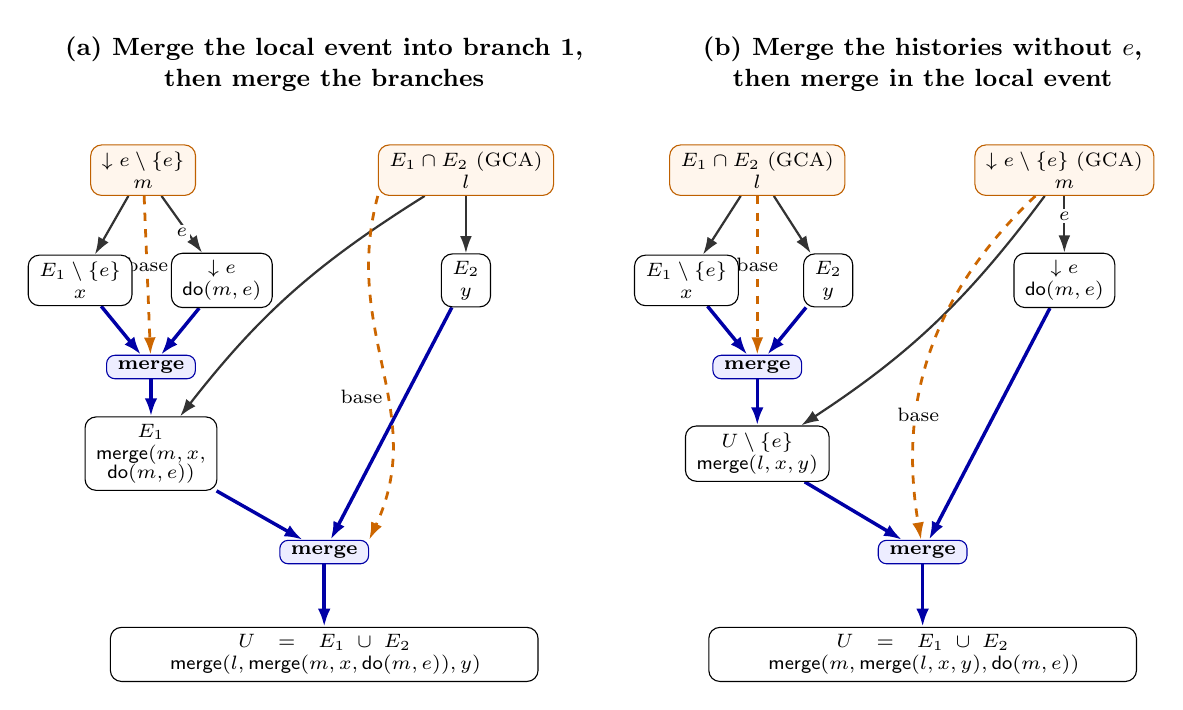
\begin{tikzpicture}[
  state/.style={draw,rounded corners,align=center,inner xsep=4pt,
    inner ysep=2.5pt,font=\scriptsize,fill=white},
  terminal/.style={state,text width=5.15cm},
  gcastate/.style={state,draw=orange!75!black,fill=orange!7},
  mergegate/.style={draw=blue!65!black,fill=blue!7,rounded corners=3pt,
    font=\scriptsize\bfseries,inner xsep=4pt,inner ysep=2pt},
  history/.style={-{Latex[length=2.2mm,width=1.5mm]},line width=.8pt,
    draw=black!80},
  mergeedge/.style={-{Latex[length=2.3mm,width=1.6mm]},line width=1.25pt,
    draw=blue!65!black},
  baseedge/.style={-{Latex[length=2.2mm,width=1.5mm]},line width=1pt,
    dashed,draw=orange!80!black},
  edgelabel/.style={font=\scriptsize,fill=white,inner sep=1pt}]

  \node[align=center,font=\small\bfseries] at (3.5,6.65)
    {(a) Merge the local event into branch 1,\\then merge the branches};

  \node[gcastate] (am) at (1.2,5.3)
    {$\downarrow e\setminus\{e\}$\\$m$};
  \node[state] (ax) at (0.4,3.9)
    {$E_1\setminus\{e\}$\\$x$};
  \node[state] (ae) at (2.2,3.9)
    {$\downarrow e$\\$\doop(m,e)$};
  \node[mergegate] (amg) at (1.3,2.8) {merge};
  \node[state] (aE1) at (1.3,1.7)
    {$E_1$\\$\merge(m,x,$\\[-1pt]$\doop(m,e))$};
  \node[gcastate] (al) at (5.3,5.3)
    {$E_1\cap E_2$ (GCA)\\$l$};
  \node[state] (ay) at (5.3,3.9)
    {$E_2$\\$y$};
  \node[mergegate] (alg) at (3.5,0.45) {merge};
  \node[terminal] (aU) at (3.5,-0.85)
    {$U=E_1\cup E_2$\\
     $\merge(l,\merge(m,x,\doop(m,e)),y)$};

  \begin{scope}[on background layer]
  \draw[history] (am) -- (ax);
  \draw[history] (am) -- node[edgelabel,below] {$e$} (ae);
  \draw[mergeedge] (ax) -- (amg);
  \draw[mergeedge] (ae) -- (amg);
  \draw[baseedge] (am) -- node[edgelabel,above] {base} (amg);
  \draw[mergeedge] (amg) -- (aE1);
  \draw[history] (al) to[bend right=10] (aE1);
  \draw[history] (al) -- (ay);
  \draw[mergeedge] (aE1) -- (alg);
  \draw[mergeedge] (ay) -- (alg);
  \draw[baseedge] (al.south west) to[out=-105,in=65,looseness=1.05]
    node[pos=.58,edgelabel,left] {base} (alg.north east);
  \draw[mergeedge] (alg) -- (aU);
  \end{scope}

  \node[align=center,font=\small\bfseries] at (11.1,6.65)
    {(b) Merge the histories without $e$,\\then merge in the local event};

  \node[gcastate] (bl) at (9.0,5.3)
    {$E_1\cap E_2$ (GCA)\\$l$};
  \node[state] (bx) at (8.1,3.9)
    {$E_1\setminus\{e\}$\\$x$};
  \node[state] (by) at (9.9,3.9)
    {$E_2$\\$y$};
  \node[mergegate] (blg) at (9.0,2.8) {merge};
  \node[state] (bUm) at (9.0,1.7)
    {$U\setminus\{e\}$\\$\merge(l,x,y)$};
  \node[gcastate] (bm) at (12.9,5.3)
    {$\downarrow e\setminus\{e\}$ (GCA)\\$m$};
  \node[state] (be) at (12.9,3.9)
    {$\downarrow e$\\$\doop(m,e)$};
  \node[mergegate] (bmg) at (11.1,0.45) {merge};
  \node[terminal] (bU) at (11.1,-0.85)
    {$U=E_1\cup E_2$\\
     $\merge(m,\merge(l,x,y),\doop(m,e))$};

  \begin{scope}[on background layer]
  \draw[history] (bl) -- (bx);
  \draw[history] (bl) -- (by);
  \draw[mergeedge] (bx) -- (blg);
  \draw[mergeedge] (by) -- (blg);
  \draw[baseedge] (bl) -- node[edgelabel,above] {base} (blg);
  \draw[mergeedge] (blg) -- (bUm);
  \draw[history] (bm) -- node[edgelabel,above] {$e$} (be);
  \draw[history] (bm) to[bend left=10] (bUm);
  \draw[mergeedge] (bUm) -- (bmg);
  \draw[mergeedge] (be) -- (bmg);
  \draw[baseedge] (bm) to[bend right=28]
    node[pos=.65,edgelabel,below] {base} (bmg);
  \draw[mergeedge] (bmg) -- (bU);
  \end{scope}
\end{tikzpicture}
\caption{The local redistribution law. Each box pairs an abstract event set
(top) with its canonical state (bottom). Black arrows show event-history
extension. Thick blue arrows enter and leave explicit merge gates. Orange
dashed arrows supply the GCA state to a gate, and orange boxes identify those
GCA states. All boxes are proof-level canonical states; the law does not
require all of them to be allocated versions in one execution. Panel (a)
constructs the $E_1$ state before the outer merge. Panel (b) first constructs
the $U\setminus\{e\}$ state and then merges in $e$. Both panels flow from
top to bottom.
\lean{localRedistribute} identifies the two terminal states.}
\label{fig:local-redistribute}
\end{figure}
\clearpage

For an event shared by both branches,
\[
\begin{gathered}
 \mathsf{redistribute}:\\[-0.3em]
\begin{aligned}
 &\forall R,E_1,E_2,m,x_0,x_1,x_2,e.\\
 &\mathsf{Admissible}_R(E_1,E_2)
   \land e\in E_1\cap E_2
   \land\mathsf{Maximal}_{R,E_1\cup E_2}(e)\\
 &\land\Can(R,(E_1\cap E_2)\setminus\{e\},x_0)
   \land\Can(R,\downarrow e\setminus\{e\},m)\\
 &\land\Can(R,E_1\setminus\{e\},x_1)
   \land\Can(R,E_2\setminus\{e\},x_2)\\
 &\Longrightarrow
 \merge(\merge(m,x_0,\doop(m,e)),
        \merge(m,x_1,\doop(m,e)),
        \merge(m,x_2,\doop(m,e)))\\
 &\hspace{5em}=
 \merge(m,\merge(x_0,x_1,x_2),\doop(m,e)).
\end{aligned}
\end{gathered}
\]
This equation extracts one shared maximal event from all three merge
components.  The feasibility restrictions exclude representation states that
no event history constructs.
\anchor{Sal/MRDTs/Framework/MergeLaws.lean}{FeasibleDeltaLaws}

Figure~\ref{fig:redistribute} presents the two sides of \lean{redistribute}
as alternative factorizations of the same union history.



\begin{figure}[htp]
\centering
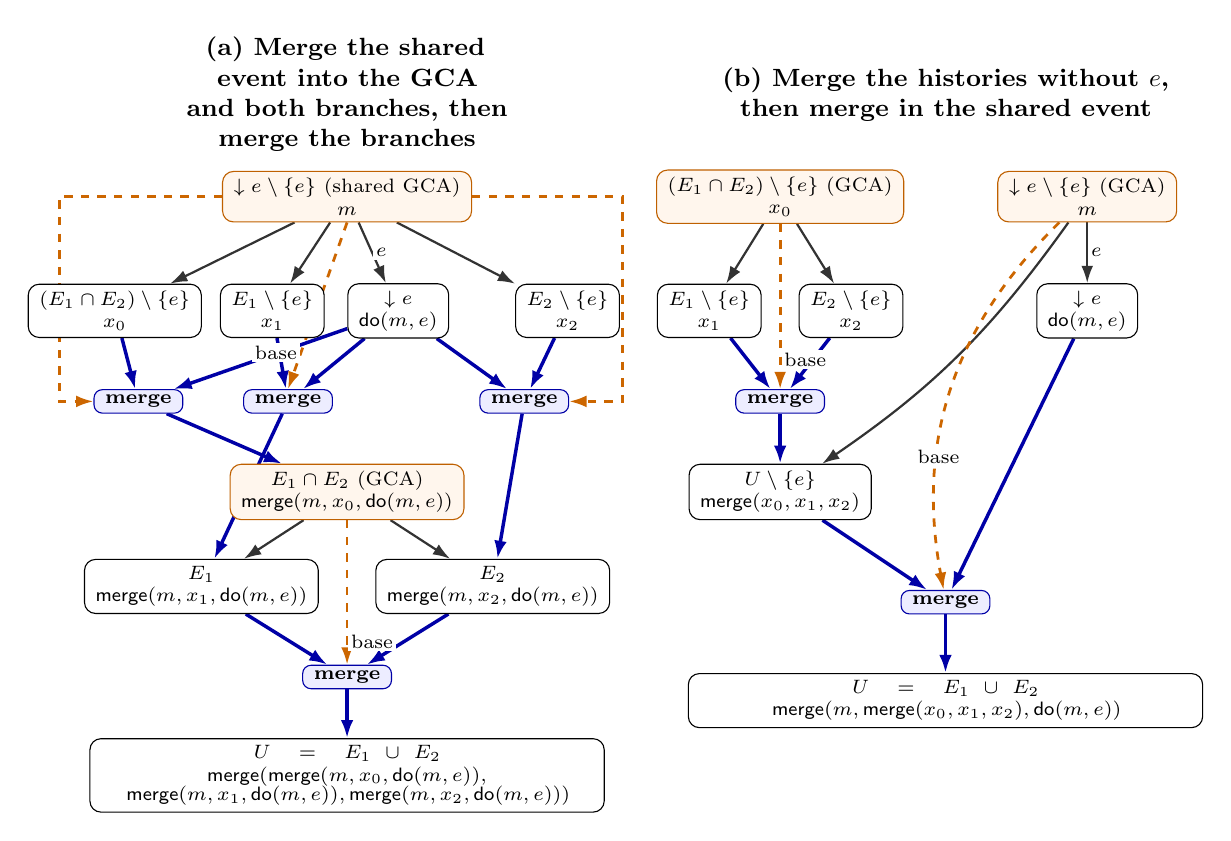
\begin{tikzpicture}[
  state/.style={draw,rounded corners,align=center,inner xsep=4pt,
    inner ysep=2.5pt,font=\scriptsize,fill=white},
  terminal/.style={state,text width=6.25cm},
  gcastate/.style={state,draw=orange!75!black,fill=orange!7},
  mergegate/.style={draw=blue!65!black,fill=blue!7,rounded corners=3pt,
    font=\scriptsize\bfseries,inner xsep=4pt,inner ysep=2pt},
  history/.style={-{Latex[length=2.2mm,width=1.5mm]},line width=.8pt,
    draw=black!80},
  mergeedge/.style={-{Latex[length=2.3mm,width=1.6mm]},line width=1.25pt,
    draw=blue!65!black},
  baseedge/.style={-{Latex[length=2.2mm,width=1.5mm]},line width=1pt,
    dashed,draw=orange!80!black},
  edgelabel/.style={font=\scriptsize,fill=white,inner sep=1pt}]

  \node[align=center,font=\small\bfseries,text width=6.5cm] at (3.5,8.7)
    {(a) Merge the shared event into the GCA\\
     and both branches, then merge the branches};

  \node[gcastate] (ram) at (3.5,7.4)
    {$\downarrow e\setminus\{e\}$ (shared GCA)\\$m$};
  \node[state] (raxz) at (0.55,5.95)
    {$(E_1\cap E_2)\setminus\{e\}$\\$x_0$};
  \node[state] (raxo) at (2.55,5.95)
    {$E_1\setminus\{e\}$\\$x_1$};
  \node[state] (rac) at (4.15,5.95)
    {$\downarrow e$\\$\doop(m,e)$};
  \node[state] (raxt) at (6.30,5.95)
    {$E_2\setminus\{e\}$\\$x_2$};
  \node[mergegate] (ragz) at (0.85,4.8) {merge};
  \node[mergegate] (rago) at (2.75,4.8) {merge};
  \node[mergegate] (ragt) at (5.75,4.8) {merge};
  \node[gcastate] (raI) at (3.5,3.65)
    {$E_1\cap E_2$ (GCA)\\$\merge(m,x_0,\doop(m,e))$};
  \node[state] (raEo) at (1.65,2.45)
    {$E_1$\\$\merge(m,x_1,\doop(m,e))$};
  \node[state] (raEt) at (5.35,2.45)
    {$E_2$\\$\merge(m,x_2,\doop(m,e))$};
  \node[mergegate] (rag) at (3.5,1.3) {merge};
  \node[terminal] (raU) at (3.5,0.05)
    {$U=E_1\cup E_2$\\
     $\merge(\merge(m,x_0,\doop(m,e)),$\\[-1pt]
     $\merge(m,x_1,\doop(m,e)),\merge(m,x_2,\doop(m,e)))$};

  \begin{scope}[on background layer]
  \draw[history] (ram) -- (raxz);
  \draw[history] (ram) -- (raxo);
  \draw[history] (ram) -- node[edgelabel,right] {$e$} (rac);
  \draw[history] (ram) -- (raxt);
  \draw[mergeedge] (raxz) -- (ragz);
  \draw[mergeedge] (rac) -- (ragz);
  \draw[mergeedge] (raxo) -- (rago);
  \draw[mergeedge] (rac) -- (rago);
  \draw[mergeedge] (raxt) -- (ragt);
  \draw[mergeedge] (rac) -- (ragt);
  \draw[baseedge] (ram.west) -- (-0.15,7.4) |- (ragz.west);
  \draw[baseedge] (ram.south) --
    node[pos=.78,edgelabel,left] {base} (rago.north);
  \draw[baseedge] (ram.east) -- (7.0,7.4) |- (ragt.east);
  \draw[mergeedge] (ragz) -- (raI);
  \draw[mergeedge] (rago) -- (raEo);
  \draw[mergeedge] (ragt) -- (raEt);
  \draw[history] (raI) -- (raEo);
  \draw[history] (raI) -- (raEt);
  \draw[mergeedge] (raEo) -- (rag);
  \draw[mergeedge] (raEt) -- (rag);
  \draw[baseedge] (raI) --
    node[pos=.84,edgelabel,right] {base} (rag);
  \draw[mergeedge] (rag) -- (raU);
  \end{scope}

  \node[align=center,font=\small\bfseries,text width=6.2cm] at (11.1,8.7)
    {(b) Merge the histories without $e$,\\
     then merge in the shared event};

  \node[gcastate] (rbxz) at (9.0,7.4)
    {$(E_1\cap E_2)\setminus\{e\}$ (GCA)\\$x_0$};
  \node[state] (rbxo) at (8.1,5.95)
    {$E_1\setminus\{e\}$\\$x_1$};
  \node[state] (rbxt) at (9.9,5.95)
    {$E_2\setminus\{e\}$\\$x_2$};
  \node[mergegate] (rbgz) at (9.0,4.8) {merge};
  \node[state] (rbUm) at (9.0,3.65)
    {$U\setminus\{e\}$\\$\merge(x_0,x_1,x_2)$};
  \node[gcastate] (rbm) at (12.9,7.4)
    {$\downarrow e\setminus\{e\}$ (GCA)\\$m$};
  \node[state] (rbc) at (12.9,5.95)
    {$\downarrow e$\\$\doop(m,e)$};
  \node[mergegate] (rbg) at (11.1,2.25) {merge};
  \node[terminal] (rbU) at (11.1,1.0)
    {$U=E_1\cup E_2$\\
     $\merge(m,\merge(x_0,x_1,x_2),\doop(m,e))$};

  \begin{scope}[on background layer]
  \draw[history] (rbxz) -- (rbxo);
  \draw[history] (rbxz) -- (rbxt);
  \draw[mergeedge] (rbxo) -- (rbgz);
  \draw[mergeedge] (rbxt) -- (rbgz);
  \draw[baseedge] (rbxz) --
    node[pos=.82,edgelabel,right] {base} (rbgz);
  \draw[mergeedge] (rbgz) -- (rbUm);
  \draw[history] (rbm) -- node[edgelabel,right] {$e$} (rbc);
  \draw[history] (rbm) to[bend left=10] (rbUm);
  \draw[mergeedge] (rbUm) -- (rbg);
  \draw[mergeedge] (rbc) -- (rbg);
  \draw[baseedge] (rbm) to[bend right=28]
    node[pos=.65,edgelabel,below] {base} (rbg);
  \draw[mergeedge] (rbg) -- (rbU);
  \end{scope}
\end{tikzpicture}
\caption{The shared redistribution law. Each box pairs an abstract event set
(top) with its canonical state (bottom). Black arrows show event-history
extension. Thick blue arrows enter and leave explicit merge gates. Orange
dashed arrows supply the GCA state, and orange boxes identify GCA states.
Panel (a) uses the same state $m$ as the base of three inner merges, producing
the branch intersection and the two branch states before the outer merge.
Panel (b) first constructs $U\setminus\{e\}$ at base $x_0$, then merges it
with $\downarrow e$ at base $m$. The fan-out edges in panel (a) reuse the
same $m$ and $\doop(m,e)$ states. Both panels flow from top to bottom, and
\lean{redistribute} identifies their terminal states.}
\label{fig:redistribute}
\end{figure}
\clearpage

The last component peels the selected maximal event from the target union.
\[
\begin{aligned}
 \mathsf{CausalDeltaLaw}(D)\Longleftrightarrow
 \forall R,U,A,B,e.\quad
 &\mathsf{Admissible}_R(U)
 \land\mathsf{Maximal}_{R,U}(e)\\
 &\land\Can(R,U\setminus\{e\},A)
 \land\Can(R,\downarrow e\setminus\{e\},B)\\
 &\Longrightarrow
 \merge(B,A,\doop(B,e))=\doop(A,e).
\end{aligned}
\]
Here $A$ represents the remaining history and $B$ represents the event's
noncommuting dependency past.
\anchor{Sal/MRDTs/Framework/MergeLaws.lean}{CausalDeltaLaw}

The single instance-facing bundle is
\[
\begin{aligned}
 \mathsf{CanonicalJoinLaws}(D)=\langle
 &\mathsf{core}:\mathsf{JoinCoreLaws}(D),\\
 &\mathsf{delta}:\mathsf{FeasibleDeltaLaws}(D),\\
 &\mathsf{causalDelta}:\mathsf{CausalDeltaLaw}(D)\rangle.
\end{aligned}
\]
Its primary theorem is
\[
 \mathsf{CanonicalJoinLaws}(D)\Longrightarrow\mathsf{Join}(D,P).
\]
The proof inducts on the union history. The empty case uses the canonical unit
law. A maximal event local to one branch uses \lean{localRedistribute}; a
maximal event shared by both branches uses \lean{redistribute}. Both cases use
\lean{CausalDeltaLaw} to peel the selected event.
\anchor{Sal/MRDTs/Framework/MergeLaws.lean}{CanonicalJoinLaws}
\anchor{Sal/MRDTs/Metatheory/Adequacy.lean}
  {CanonicalJoinLaws.join, JoinProof.ofFeasibleStateLaws}

\subsubsection{Universal equations as a shortcut}

Many datatypes satisfy stronger equations for arbitrary representation
states. The universal merge bundle \lean{MergeLaws} contains only the fields
used by the universal-to-canonical bridge:
\[
\begin{aligned}
 \mathsf{MergeLaws}(D)=\langle
 &\mathsf{replay}:\mathsf{ReplayLaws}(D,P),\\
 &\mathsf{mergeComm}:\forall l,a,b.\;
   \merge(l,a,b)=\merge(l,b,a),\\
 &\mathsf{mergeInit}:\forall s.\;
   \merge(\init,\init,s)=s\rangle.
\end{aligned}
\]
\anchor{Sal/MRDTs/Framework/MergeLaws.lean}{MergeLaws}

The bundle \lean{DeltaLaws} contains the two universal delta equations. Here
$c$ is an arbitrary state; the canonical adapter substitutes
$\doop(m,e)$ for it.
\[
\begin{aligned}
 \merge(\merge(m,x_0,c),\merge(m,x_1,c),\merge(m,x_2,c))
   &=\merge(m,\merge(x_0,x_1,x_2),c),\\
 \merge(l,\merge(m,x,c),y)&=\merge(m,\merge(l,x,y),c).
\end{aligned}
\]
\anchor{Sal/MRDTs/Framework/MergeLaws.lean}{DeltaLaws}

The auxiliary \lean{CommutingPeelLaw} states that an update can be pulled
through a merge when it commutes with every event replayed in the other two
components:
\[
\begin{aligned}
 &\mathsf{CommutingPeelLaw}(D)\Longleftrightarrow\\
 &\quad\forall a,e,\pi_0,\pi_2.\quad
 \left(\forall x\in\pi_0.\;e\leftrightarrow x\right)
 \land\left(\forall x\in\pi_2.\;e\leftrightarrow x\right)\\
 &\quad\Longrightarrow
 \merge\bigl(\applySeq(D,\init,\pi_0),\doop(a,e),
                   \applySeq(D,\init,\pi_2)\bigr)\\
 &\qquad\quad=
 \doop\Bigl(\merge\bigl(\applySeq(D,\init,\pi_0),a,
                         \applySeq(D,\init,\pi_2)\bigr),e\Bigr).
\end{aligned}
\]
This auxiliary adapter sits outside the canonical Join contract. Together
with \lean{MergeLaws} and universal update commutativity, it supplies
\lean{CausalDeltaLaw} for the all-commuting instance class.
\[
\begin{aligned}
 \mathsf{MergeLaws}(D)&+\mathsf{CommutingPeelLaw}(D)
 +(\forall e,e'.\;e\leftrightarrow e')\\
 &\Longrightarrow\mathsf{CausalDeltaLaw}(D).
\end{aligned}
\]
\anchor{Sal/MRDTs/Framework/MergeLaws.lean}{CommutingPeelLaw}
\anchor{Sal/MRDTs/Metatheory/Adequacy.lean}
  {causalDeltaLaw\_of\_all\_comm}

RGA satisfies these universal equations by pointwise Boolean identities.
The adapter details are in Appendix~\ref{app:merge-adapters}; the resulting
merge theorem holds for every replay context. Issuance is used separately
to construct the legal ordinary-list witness.
\anchor{Sal/MRDTs/Instances/RGA.lean}{RGA.join}

\subsection{Ordinary adequacy}

The initial configuration is canonical. Fork copies a canonical version;
apply extends one with a fresh maximal event; query stutters; and merge is the
Join implication after the GCA theorem identifies the base set with
$E_1\cap E_2$. Write
$\mathsf{Reachable}(\mathsf{Step},C_0,C)$ for the reflexive-transitive closure
of the raw transition relation. Hence
\[
 \mathsf{Join}(D,P)\to
 \mathsf{Reachable}(\mathsf{Step},\mathsf{initConfig}(D),C)
 \to\mathsf{HasReplayWitness}(C).
\]
The proof establishes \lean{CanonicalConfig C} first and projects replay only
at the end.
\anchor{Sal/MRDTs/Metatheory/Adequacy.lean}{replayWitness\_of\_join}

\section{Issuance and client-facing correctness}
\label{sec:client}

Fix a datatype $D$ with operations $O$, concrete state $\State$, query type
$Q$, and result type $R$, and a replay policy $P$ supplying its resolve-conflict
relation $rc$. We first define the sequential behavior against which $D$ is
checked, then the executions to which the correctness claim applies.

\subsection{Sequential specification}

A sequential specification $\mathit{Spec}$ contains
\[
\begin{array}{rcl}
 \State_S&:&\mathsf{Type},\\
 \sigma^S_0&:&\State_S,\\
 \mathsf{step}_S&:&\State_S\to\Event(O)\to\State_S,\\
 \mathsf{Legal}_S&:&\mathsf{List}(\Event(O))\to\mathsf{Prop},\\
 \query_S&:&\State_S\to Q\to R.
\end{array}
\]
Its run is the left fold of $\mathsf{step}_S$ from $\sigma^S_0$.
The predicate $\mathsf{Legal}_S$ constrains the event list; it receives
neither the implementation state nor visibility. The witness must separately
respect $\loOn$, defined in Section~\ref{sec:rc-order}. Legality may further
constrain its order: TreeMove, for example, requires a key-sorted list.
\anchor{Sal/MRDTs/Framework/Certificates.lean}
  {SequentialMachine, SequentialSpec, SequentialSpec.run}

Choose a representation relation
$\mathsf{Rel}:\State\to\State_S\to\mathsf{Prop}$.
For a configuration $C$, write $S$ for its version store and $R_C$ for its
replay context, as in the preceding sections.

\begin{definition}[Client-facing linearizability]
$\mathsf{IsSpecLinearizable}(D,P,\mathit{Spec},\mathsf{Rel},C)$ means
\[
\begin{aligned}
 \forall v,s,E.\;S(v)=(s,E)\to\exists\pi.\;&
 \mathsf{listPermOf}(\pi,E)\\
 &\land\mathsf{respects}
   (\pi,\lambda e_1\,e_2.\;e_1\;\loOn_{R_C,E}\;e_2)\\
 &\land \mathit{Spec}.\mathsf{Legal}(\pi)\\
 &\land\mathsf{Rel}(s,\mathit{Spec}.\mathsf{run}(\pi))\\
 &\land\forall q.\;D.\query(s,q)=
   \mathit{Spec}.\query(\mathit{Spec}.\mathsf{run}(\pi),q).
\end{aligned}
\]
Here $\loOn$ uses the fixed policy $P$.
\anchor{Sal/MRDTs/Metatheory/Correctness.lean}{IsSpecLinearizable}
\end{definition}

For each stored version, one and the same list must enumerate exactly its
events, respect $\loOn$, satisfy the sequential legality condition, relate
the two states, and give the same answer to every query. The specification
and relation are part of the datatype's contract, not consequences of a
replay proof.

\subsection{Issuance and certified execution}

An issuance policy $I$ contains
\[
 I.\mathsf{CanIssue}:\Event(O)\to\State\to\mathsf{Prop}.
\]
It states when an event may be created at an issuing replica's concrete
state. For configurations $C,C'$ and a transition label $\ell$,
$\mathsf{IssuedStep}(D,I,C,\ell,C')$ is defined by the following rules,
where $H$ and $S$ are the head map and version store of $C$:
\[
\frac{
  \mathsf{Step}(D,C,\ell,C')\qquad
  \forall t,r,o.\;\ell\ne\mathsf{apply}(t,r,o)
}{
  \mathsf{IssuedStep}(D,I,C,\ell,C')
}\;\textsc{Non-apply}
\]
\[
\frac{
  \begin{gathered}
  H(r)=v\qquad S(v)=(s,E)\qquad
  I.\mathsf{CanIssue}((t,r,o),s)\\
  \mathsf{Step}(D,C,\mathsf{apply}(t,r,o),C')
  \end{gathered}
}{
  \mathsf{IssuedStep}(D,I,C,\mathsf{apply}(t,r,o),C')
}\;\textsc{Apply}
\]
Fork, merge, and query add no issuance check. Apply checks the actual
issuing head state, in addition to the raw transition's premises.
\anchor{Sal/MRDTs/Framework/Certificates.lean}{Issuance, IssuedStep}

A separate condition, $\mathsf{MintHonest}$, requires each event to be
issuable after some visibility-respecting enumeration of its causal past:
\[
\begin{aligned}
 &\mathsf{MintHonest}(D,I.\mathsf{CanIssue},C)\Longleftrightarrow\\
 &\quad\forall e\in C.\mathsf{events}.\;\exists\pi.\;
 \mathsf{listPermOf}(\pi,\{e'\in C.\mathsf{events}\mid e'\vis e\})\\
 &\qquad\land\mathsf{respects}(\pi,\vis)
 \land I.\mathsf{CanIssue}(e,\applySeq(D,\init,\pi)).
\end{aligned}
\]
This is an existential condition on the causal past, not a check at the
stored issuing head. Its enumeration respects full visibility, whereas
the client witness above respects $\loOn$.
\anchor{Sal/MRDTs/Framework/Certificates.lean}{MintHonest}

Certified reachability $\mathsf{MintCertifiedReach}(D,I,C)$ has an initial
case $\mathsf{MintCertifiedReach}(D,I,\mathsf{initConfig}(D))$ and the step rule
\[
\frac{
 \begin{gathered}
 \mathsf{MintCertifiedReach}(D,I,C)\qquad
 \mathsf{IssuedStep}(D,I,C,\ell,C')\\
 \mathsf{MintHonest}(D,I.\mathsf{CanIssue},C)\qquad
 \mathsf{MintHonest}(D,I.\mathsf{CanIssue},C')
 \end{gathered}
}{
 \mathsf{MintCertifiedReach}(D,I,C')
}.
\]
Thus the definition requires mint honesty before and after each step.
It does not derive this condition merely from the local issuance checks.
A claim covering all executions that obey those checks would additionally
need to establish this provenance condition.
\anchor{Sal/MRDTs/Framework/Certificates.lean}{MintCertifiedReach}

Erasing these premises recovers raw reachability:
\[
 \mathsf{MintCertifiedReach}(D,I,C)
 \Longrightarrow
 \mathsf{Reachable}(\mathsf{Step},\mathsf{initConfig}(D),C).
\]
\anchor{Sal/MRDTs/Framework/Certificates.lean}
  {MintCertifiedReach.toReachable}

\subsection{Correctness obligation}

For the chosen $D$, $P$, $I$, $\mathit{Spec}$, and $\mathsf{Rel}$, the
ordinary-execution correctness obligation is
\[
 \forall C.\;
 \mathsf{MintCertifiedReach}(D,I,C)
 \Longrightarrow
 \mathsf{IsSpecLinearizable}(D,P,\mathit{Spec},\mathsf{Rel},C).
\]
This implication must be proved for the chosen contract; it does not follow
from the interface definitions alone. In particular,
$\mathsf{HasReplayWitness}(C)$ only provides an ordering whose concrete fold
is the stored state. It does not by itself establish sequential legality,
the representation relation, or agreement with the abstract queries.

The next section extends execution to synthetic merge bases.
Section~\ref{sec:certificates} packages the proofs for both execution
semantics and describes sufficient proof routes.

\section{Canonical virtual merge bases}
\label{sec:virtual}

An execution DAG need not have a GCA for every pair. The widened
semantics supplies a synthetic base state computed from the antichain of
maximal common ancestors. No synthetic base version is allocated.

\subsection{Resolver and widened merge}

A resolver $V$ contains
\[
 V.\mathsf{state}:\mathsf{Configuration}(D)\to\Version\to\Version\to\State.
\]
\lean{StepV D V} includes every ordinary step through \lean{base} and one
additional merge constructor. For head states $s_1,s_2$, its new-version
equation is
\[
 S'(v_m)=
 (\merge(V.\mathsf{state}(C,v_1,v_2),s_1,s_2),E_1\cup E_2),
\]
with the same head, parent, freshness, and rank updates as ordinary merge. It
does not require a GCA.
\anchor{Sal/MRDTs/Framework/Execution.lean}
  {VirtualMergeBaseResolver, StepV, StepV.mergeVirtual}

\lean{IssuedStepV D V I} embeds an ordinary issued step or accepts a genuinely
virtual \lean{StepV} derivation that is not an ordinary \lean{Step}.
\lean{MintCertifiedReachV D V I C} is its inductive closure from the initial
configuration, retaining mint honesty before and after every step.
\anchor{Sal/MRDTs/Framework/Certificates.lean}
  {IssuedStepV, MintCertifiedReachV}

\subsection{Recursive maximal-ancestor fold}

The recursive fold needs a generalization of the pairwise definition. For a
finite support $X$, let
\[
\begin{aligned}
 \mathsf{CAWithAny}_P(X,w)
   &=\bigcup_{u\in X}\mathsf{CommonAncestors}(P,u,w),\\
 \mathsf{IsMaximalWithAny}_P(X,w,m)
   &\Longleftrightarrow
     m\in\mathsf{CAWithAny}_P(X,w)\\
   &\quad\land
     \forall x\in\mathsf{CAWithAny}_P(X,w).\;
       m\reach x\to x=m.
\end{aligned}
\]
In other words, a candidate must be a common ancestor of $w$ and at least one
member of $X$; it need not be an ancestor of every member of $X$. Lean names
these definitions \lean{CommonAncestorsWithAny} and
\lean{IsMaximalCommonAncestorWithAny}. Write
\[
 \mathsf{BasesWithAny}(P,X,w)
 =\{m\mid
   \mathsf{IsMaximalWithAny}_P(X,w,m)\}
\]
for the finite enumeration implemented by
\lean{maximalCommonAncestorsWithAny}. The singleton bridge is
\[
 \mathsf{IsMaximalWithAny}_P(\{a\},b,m)
 \Longleftrightarrow
 \mathsf{IsMaximalCommonAncestor}(P,a,b,m).
\]
\anchor{Sal/MRDTs/Framework/Execution.lean}
  {CommonAncestorsWithAny, IsMaximalCommonAncestorWithAny,
   isMaximalCommonAncestorWithAny\_singleton}
\anchor{Sal/MRDTs/Metatheory/VirtualMergeBase.lean}
  {maximalCommonAncestorsWithAny,
   mem\_maximalCommonAncestorsWithAny\_iff}

Sort $\mathsf{BasesWithAny}(P,X,w)$ by increasing version rank. Let
$\mathsf{stateD}(v)$ return the stored state, defaulting to $\init$ only to
make the function total. Define the scratch fold $\mathsf{vfold}$ and its
recursive base resolver $\mathsf{vbase}$ mutually:
\[
\begin{aligned}
 \mathsf{vfold}(A,a,[])&=a,\\
 \mathsf{vfold}(A,a,m::ms)&=
 \mathsf{vfold}\bigl(A\cup\{m\},
   \merge(\mathsf{vbase}(A,m),a,\mathsf{stateD}(m)),ms\bigr).
\end{aligned}
\]
The nested base is itself the fold of this sorted maximal antichain:
\[
 \mathsf{vbase}(X,w)=
 \begin{cases}
 \init,&\mathsf{sort}(\mathsf{BasesWithAny}(P,X,w))=[],\\
 \mathsf{vfold}(\{m_1\},\mathsf{stateD}(m_1),ms),
   &\mathsf{sort}(\mathsf{BasesWithAny}(P,X,w))=m_1::ms.
 \end{cases}
\]
Termination uses the cardinality of the joint ancestor support,
lexicographically paired with pending-list length. The head-pair resolver is
\[
 \mathsf{virtualMergeBaseState}(C,v_1,v_2)=\mathsf{vbase}(\{v_1\},v_2).
\]
The resolver whose $\mathsf{state}$ field is this function is
$\mathsf{canonicalVirtualMergeBase}(D)$.
\anchor{Sal/MRDTs/Metatheory/VirtualMergeBase.lean}
  {vfoldAux, virtualBaseAux, virtualMergeBaseState, canonicalVirtualMergeBase}

\subsection{Virtual canonicity and adequacy}

For finite $X\subseteq A_C$,
\[
 \mathsf{unionEvents}(C,X)=
 \bigcup_{v\in X}\mathsf{events}_C(v).
\]
Under \lean{StoreInv}, for allocated $w$, the maximal-base event union is
exactly the outer intersection:
\[
 \mathsf{unionEvents}(C,\mathsf{BasesWithAny}(P,X,w))
 =\mathsf{unionEvents}(C,X)\cap\mathsf{events}_C(w).
\]
\anchor{Sal/MRDTs/Metatheory/VirtualAdequacy.lean}
  {unionEvents, maximalCommonAncestorsWithAny\_unionEvents}

The fold theorem states
\[
\begin{aligned}
 &\mathsf{StoreInv}(S,P)\land\mathsf{CanonicalConfig}(C)
 \land\mathsf{JoinAt}(D,P,R_C)\\
 &\land S(v_1)=(s_1,E_1)\land S(v_2)=(s_2,E_2)\\
 &\Longrightarrow
 \Can(R_C,E_1\cap E_2,\mathsf{virtualMergeBaseState}(C,v_1,v_2)).
\end{aligned}
\]
\anchor{Sal/MRDTs/Metatheory/VirtualAdequacy.lean}
  {virtualMergeBaseState\_canonical}

Consequently,
\[
\begin{aligned}
 \mathsf{Join}(D,P)&\to
 \mathsf{Reachable}(\mathsf{StepV},
   \mathsf{initConfig}(D),C)
 \to\mathsf{CanonicalConfig}(C),\\
 \mathsf{Join}(D,P)&\to
 \mathsf{Reachable}(\mathsf{StepV},
   \mathsf{initConfig}(D),C)
 \to\mathsf{HasReplayWitness}(C).
\end{aligned}
\]
\anchor{Sal/MRDTs/Metatheory/VirtualAdequacy.lean}
  {canonicalConfig\_reachableV, replayWitnessV\_of\_join}

As in the ordinary semantics, certified widened reachability erases to raw
widened reachability. Hence the all-context Join theorem also supplies
replay witnesses for certified widened executions.
\anchor{Sal/MRDTs/Framework/Certificates.lean}
  {MintCertifiedReachV.toReachable}

\subsection{Verification certificates}
\label{sec:certificates}

A replay-adequacy certificate
$\mathsf{ReplayAdequacyCertificate}(D,I,P)$ has field
\[
 \mathsf{soundV}:\quad
 \mathsf{MintCertifiedReachV}(D,\mathsf{canonicalVirtualMergeBase}(D),I,C)
 \to\mathsf{HasReplayWitness}(C).
\]
Ordinary soundness follows because ordinary execution embeds in widened
execution.
\anchor{Sal/MRDTs/Metatheory/Correctness.lean}
  {ReplayAdequacyCertificate, ReplayAdequacyCertificate.sound}

For a context predicate $G:\mathsf{ReplayContext}(D)\to\mathsf{Prop}$,
define
\[
 \mathsf{IssuanceEstablishes}(D,I,G)\Longleftrightarrow
 \forall C.\;\mathsf{MintHonest}(D,I.\mathsf{CanIssue},C)
 \to G(R_C).
\]
This is a proof obligation from mint honesty to $G$, not a theorem deriving
mint honesty from local issuance checks.
\anchor{Sal/MRDTs/Framework/Certificates.lean}{IssuanceEstablishes}

The artifact provides two sufficient constructors:
\[
\begin{aligned}
 \mathsf{Join}(D,P)
 &\Longrightarrow \mathsf{ReplayAdequacyCertificate}(D,I,P),\\
 \mathsf{JoinOn}(D,P,G)
 \land\mathsf{IssuanceEstablishes}(D,I,G)
 &\Longrightarrow \mathsf{ReplayAdequacyCertificate}(D,I,P).
\end{aligned}
\]
The first constructor erases certified widened reachability before applying
all-context Join; the second uses issuance consistency to discharge the explicit
context condition.
\anchor{Sal/MRDTs/Metatheory/Correctness.lean}
  {ReplayAdequacyCertificate.ofJoin}
\anchor{Sal/MRDTs/Metatheory/Correctness.lean}
  {ReplayAdequacyCertificate.ofJoinOn}

The first accepts any issuance policy. For the second, certified reachability
supplies mint honesty at each configuration; the separate proof of
$\mathsf{IssuanceEstablishes}$ supplies $G(R_C)$, and
$\mathsf{JoinOn}(D,P,G)$ supplies the required local merge theorem.
For ordinary executions, the premises compose as
\[
\begin{aligned}
 &\mathsf{JoinOn}(D,P,G)\land\mathsf{IssuanceEstablishes}(D,I,G)\\
 &\land\mathsf{MintCertifiedReach}(D,I,C)\\
 &\qquad\Longrightarrow\mathsf{HasReplayWitness}(C).
\end{aligned}
\]
The corresponding widened theorem replaces the third premise with
$\mathsf{MintCertifiedReachV}
(D,\mathsf{canonicalVirtualMergeBase}(D),I,C)$.
\anchor{Sal/MRDTs/Metatheory/CertifiedAdequacy.lean}
  {replayWitness\_of\_mintCertified, replayWitness\_of\_mintCertifiedV}

These constructors do not exhaust the possible proofs: an instance may
prove the replay-adequacy field directly by an execution invariant.

Let $\mathsf{CertifiedExecution}(D,I,C)$ mean either an ordinary
$\mathsf{MintCertifiedReach}(D,I,C)$ derivation or a widened
$\mathsf{MintCertifiedReachV}
(D,\mathsf{canonicalVirtualMergeBase}(D),I,C)$ derivation. A
sequential-correctness certificate has type
\[
 \forall C.\;\mathsf{CertifiedExecution}(D,I,C)
 \to\mathsf{HasReplayWitness}(C)
 \to\mathsf{IsSpecLinearizable}(D,P,\mathit{Spec},\mathsf{Rel},C).
\]
\anchor{Sal/MRDTs/Metatheory/Correctness.lean}
  {CertifiedExecution, SequentialCorrectnessCertificate}

The complete package is
\[
\begin{aligned}
 \mathsf{VerifiedMRDT}(D)=(&I:\mathsf{Issuance}(D),\\
 &rc:\mathsf{ReplayPolicy}(D),\\
 &K:\mathsf{ReplayAdequacyCertificate}(D,I,rc),\\
 &\mathit{Spec}:\mathsf{SequentialSpec}(D),\\
 &\mathsf{Rel}:\State\to\State_S\to\mathsf{Prop},\\
 &K_S:\mathsf{SequentialCorrectnessCertificate}
   (D,I,rc,\mathit{Spec},\mathsf{Rel})).
\end{aligned}
\]
\lean{PackagedMRDT} additionally contains a name and the signature $D$.
\anchor{Sal/MRDTs/Metatheory/Correctness.lean}
  {VerifiedMRDT, PackagedMRDT}

Its public conclusions are
\[
\begin{aligned}
 \mathsf{MintCertifiedReach}(D,I,C)&\to
   \mathsf{IsSpecLinearizable}(D,rc,\mathit{Spec},\mathsf{Rel},C),\\
 &\mathsf{MintCertifiedReachV}
   (D,\mathsf{canonicalVirtualMergeBase}(D),I,C)\\
 &\qquad\to
   \mathsf{IsSpecLinearizable}(D,rc,\mathit{Spec},\mathsf{Rel},C).
\end{aligned}
\]
\anchor{Sal/MRDTs/Metatheory/Correctness.lean}
  {VerifiedMRDT.correct, VerifiedMRDT.correctV}

\section{Distributed commit-history collection}
\label{sec:history-gc}

Replicas fetch commits asynchronously, so each replica decides locally when
history can be removed. It must retain enough authored evidence and enough
graph information for future reachability and merge-base queries.

\subsection{Local holdings and evidence}

A local holding is
\[
 \mathsf{Local}=(\mathsf{head}:\Version,
   \mathsf{commits}:\Pow(\Version),
   \mathsf{headPresent}:\mathsf{head}\in\mathsf{commits}).
\]
An envelope contains a commit set. Advertising exports the local set;
receiving unions it into the destination without changing the head. A world is
$\mathsf{World}=\Replica\to\mathsf{Local}$.
\anchor{Sal/MRDTs/GC/Distributed.lean}
  {GC.Local, GC.Envelope, GC.advertise, GC.receive, GC.World}

Authorship has type
$\mathsf{Author}=\Version\to\mathsf{Option}(\Replica)$. Evidence for roster
member $r$ is
\[
\begin{aligned}
 \mathsf{DerivedEvidence}(P,A,L,r)=\{v\mid{}&
 v\in L.\mathsf{commits}\land A(v)=r\\
 &\land\mathsf{Reaches}(P,v,L.\mathsf{head})\}.
\end{aligned}
\]
Evidence is complete for roster $R$ at replica $r_s$ when
\[
\begin{aligned}
 \mathsf{EvidenceComplete}(P,A,R,r_s,L)\Longleftrightarrow
 \forall r\in R.\;&r=r_s\lor\\
 &\exists v.\;v\in\mathsf{DerivedEvidence}(P,A,L,r).
\end{aligned}
\]
\anchor{Sal/MRDTs/GC/Distributed.lean}
  {GC.Author, GC.DerivedEvidence, GC.EvidenceComplete}

\subsection{Compression certificate}

For any reachability relation $R_V$ on versions, define
\[
\begin{aligned}
 \mathsf{IsGCARel}(R_V,v_1,v_2,v_T)\Longleftrightarrow{}&
 R_V(v_T,v_1)\land R_V(v_T,v_2)\\
 &\land\forall w.\;R_V(w,v_1)\land R_V(w,v_2)
   \to R_V(w,v_T).
\end{aligned}
\]
The canonical compressed edge summarizes any old path between retained
endpoints:
\[
 \mathsf{compressedEdge}_{P,K}(a,b)
 \Longleftrightarrow a\in K\land b\in K\land\mathsf{Reaches}(P,a,b).
\]
Define
\[
 \mathsf{CompressedReaches}_{P,K}
 =\bigl(\mathsf{compressedEdge}_{P,K}\bigr)^*.
\]
This relation preserves reachability exactly on retained nodes. Closure of
$K$ under maximal common ancestors suffices to preserve GCA answers; retaining
intermediate paths or version $0$ is unnecessary.
\anchor{Sal/MRDTs/GC/CompressedDAG.lean}
  {GC.compressedEdge, GC.CompressedReaches, GC.compressedReaches\_iff}
\anchor{Sal/MRDTs/GC/CompressedDAG.lean}
  {GC.compressed\_isGCA\_iff\_of\_\allowbreak maximalCommonAncestorClosed,
   GC.root\_absent\_when\_dropped}

A collection certificate chooses $K\subseteq L.\mathsf{commits}$ and proves:
\begin{enumerate}
\item evidence is complete, the local head is retained, and suitable evidence
  for every remote roster member is retained;
\item for $a,b\in K$,
  $\mathsf{CompressedReaches}_{P,K}(a,b)$ is equivalent to
  $\mathsf{Reaches}(P,a,b)$; and
\item for retained $v_1,v_2,v_T$,
  $\mathsf{IsGCARel}(\mathsf{CompressedReaches}_{P,K},v_1,v_2,v_T)$ is
  equivalent to $\mathsf{IsGCA}(P,v_1,v_2,v_T)$.
\end{enumerate}
Collection replaces the local commit set by $K$ and preserves its head.
\anchor{Sal/MRDTs/GC/Distributed.lean}
  {GC.Certificate, GC.collect}

Define the pairwise closure condition by
\[
\begin{aligned}
 \mathsf{MaximalClosed}_P(K)\Longleftrightarrow{}&
   \forall a,b\in K.\;\forall m.\\
 &\mathsf{IsMaximalCommonAncestor}(P,a,b,m)\to m\in K.
\end{aligned}
\]
The canonical constructor then has the schematic type
\[
\begin{aligned}
 \mathsf{ofMaximalClosed}:{}&
 \mathsf{EvidenceComplete}(P,A,R,r_s,L)
 \to L.\mathsf{head}\in K\\
 &\to(\forall r\in R.\;r=r_s\lor
   \exists v\in\mathsf{DerivedEvidence}(P,A,L,r).\;v\in K)\\
 &\to K\subseteq L.\mathsf{commits}
 \to(\forall v,p.\;p\in P(v)\to p<v)\\
 &\to\mathsf{MaximalClosed}_P(K)
 \to\mathsf{Certificate}.
\end{aligned}
\]
The exact Lean constructor is named in the source anchor.
\anchor{Sal/MRDTs/GC/Distributed.lean}
  {GC.Certificate.\allowbreak ofMaximalCommonAncestorClosed}

\subsection{Asynchronous refinement}

The collecting protocol has fetch, head synchronization, and local
collection. Its comparison protocol has fetch and head synchronization but no
collection. Define
\[
\begin{aligned}
 \mathsf{StoreSim}(F,C)\Longleftrightarrow{}&
 F.\mathsf{head}=C.\mathsf{head}\\
 &\land C.\mathsf{commits}\subseteq F.\mathsf{commits}
 \land C.\mathsf{head}\in C.\mathsf{commits},\\
 \mathsf{WorldSim}(F,C)\Longleftrightarrow{}&
 \forall r.\;\mathsf{StoreSim}(F(r),C(r)).
\end{aligned}
\]
One collecting step is matched by the corresponding network step or
stuttering. Write $\mathsf{Steps}_{GC}$ and $\mathsf{NoGCSteps}$ for the
reflexive-transitive closures of the collecting and comparison step relations,
respectively. Then
\[
\begin{aligned}
 &\mathsf{WorldSim}(F_0,C_0)\land\mathsf{Steps}_{GC}(C_0,C_1)\\
 &\qquad\Longrightarrow\exists F_1.\;
 \mathsf{NoGCSteps}(F_0,F_1)\land\mathsf{WorldSim}(F_1,C_1).
\end{aligned}
\]
\anchor{Sal/MRDTs/GC/Distributed.lean}
  {GC.StoreSim, GC.WorldSim, GC.execution\_refines\_noGC}

\section{Runtime and datatype-state collection}
\label{sec:state-gc}

\subsection{Commit-store runtime refinement}

A datatype-rich runtime pairs semantics with local stores:
\[
 \mathsf{Runtime}(D)=
 (\mathsf{core}:\mathsf{Configuration}(D),
  \mathsf{stores}:\mathsf{World}).
\]
It is well formed when each retained commit is allocated in the core and each
semantic replica head agrees with its store head. A visible runtime transition
contains an actual \lean{Step} derivation and matching store evolution. Fetch
and collection are silent.
\anchor{Sal/MRDTs/GC/Refinement.lean}
  {GC.Runtime, GC.Runtime.WellFormed, GC.RuntimeStep}

Erasing optional labels removes silent steps:
\[
 \mathsf{eraseLabels}=\mathsf{List.filterMap}(\mathsf{id}).
\]
Let $\mathsf{RuntimeSteps}$ be the list-labelled reflexive-transitive closure
of runtime transitions, and let $\mathsf{CoreSteps}$ be the corresponding
closure of raw \lean{Step} transitions. Finite runtime traces refine raw
semantic traces:
\[
 \mathsf{RuntimeSteps}(D,A,R,S_0,ls,S_1)
 \to\mathsf{CoreSteps}
   (D,S_0.\mathsf{core},\mathsf{eraseLabels}(ls),S_1.\mathsf{core}).
\]
The widened theorem uses the virtual-merge-base step relations and parameterizes
availability by the exact versions read by the resolver.
\anchor{Sal/MRDTs/GC/Refinement.lean}
  {GC.eraseLabels, GC.runtime\_refines\_core, GC.runtime\_refines\_coreV}

\subsection{Datatype-state GC}

A local collector is first specified independently of a runtime transition
system.  For an issuance policy $I$, a certificate supplies compact states
$C$, collection evidence $W$, a relation $c\mathrel{\mathsf{Rep}}s$ to the
full datatype state, an evidence predicate
$\mathsf{EvidenceValid}:W\to C\to\State\to\mathsf{Prop}$,
a branch-compatibility predicate
$\mathsf{Compatible}:\State\to\State\to\mathsf{Prop}$, and compact interpretations of
initialization, update, ternary merge, and query.  Its central obligations are
\[
\begin{aligned}
 c\mathrel{\mathsf{Rep}}s\land\mathsf{EvidenceValid}(w,c,s)
 &\Longrightarrow \mathsf{collect}(w,c)\mathrel{\mathsf{Rep}}s,\\
 c\mathrel{\mathsf{Rep}}s\land I.\mathsf{CanIssue}(e,s)
 &\Longrightarrow \mathsf{update}_C(c,e)
       \mathrel{\mathsf{Rep}}\doop(s,e),\\
 c_l\mathrel{\mathsf{Rep}}l\land c_a\mathrel{\mathsf{Rep}}a
 \land c_b\mathrel{\mathsf{Rep}}b\land\mathsf{Compatible}(a,b)
 &\Longrightarrow \mathsf{merge}_C(c_l,c_a,c_b)
       \mathrel{\mathsf{Rep}}\merge(l,a,b),\\
 c\mathrel{\mathsf{Rep}}s
 &\Longrightarrow \mathsf{query}_C(c,q)=\mathsf{query}(s,q).
\end{aligned}
\]
Together with the corresponding initialization law, this is
\lean{StateGCCertificate}.  The generic
\lean{StateGCCertificate.exactState} chooses $C=\State$, equality as
$\mathsf{Rep}$, and identity collection.  It is a preservation baseline, not
a reclamation result.

The more general \lean{StateGCProtocol} embeds collection into physical
execution.  It supplies
\[
\begin{array}{rcl}
 \mathsf{Physical}&:&\mathsf{Type},\\
 \mathsf{semantic}&:&\mathsf{Physical}\to\mathsf{Configuration}(D),\\
 \mathsf{Valid}&:&\mathsf{Physical}\to\mathsf{Prop},\\
 \mathsf{PhysicalStep}&:&\mathsf{Physical}\to
   \mathsf{Option}(\mathsf{Label}(D))\to\mathsf{Physical}\to\mathsf{Prop}.
\end{array}
\]
It proves validity preservation, silent stuttering
$\mathsf{semantic}(P')=\mathsf{semantic}(P)$, and visible refinement to
\lean{StepV D V}. Write $\mathsf{SemanticSteps}_V$ for the list-labelled
reflexive-transitive closure of \lean{StepV D V}. Every finite valid physical
trace therefore erases to such a widened semantic trace.
\anchor{Sal/MRDTs/Framework/StateGC.lean}
  {StateGCCertificate, StateGCCertificate.exactState,
   StateGCProtocol, StateGCProtocol.refines}

\subsection{Composition}

The combined physical state pairs a datatype-state physical value with a
commit world. A step is either a datatype-state step, with matching store
evolution for a visible label, or a silent history fetch/collection step.
Write $\mathsf{Combined.Valid}$ for componentwise validity and
$\mathsf{CombinedSteps}$ for the list-labelled closure of these combined
steps. \lean{combinedProtocol} is itself a \lean{StateGCProtocol}; hence
\[
\begin{aligned}
 &\mathsf{Combined.Valid}(P)\land
 \mathsf{CombinedSteps}(P,ls,P')\\
 &\qquad\Longrightarrow
 \mathsf{SemanticSteps}_V
 (\mathsf{semantic}(P),\mathsf{eraseLabels}(ls),\mathsf{semantic}(P')).
\end{aligned}
\]
If the datatype protocol also proves that every visible physical step is raw,
the ordinary refinement follows.
\anchor{Sal/MRDTs/GC/StateComposition.lean}
  {GC.combinedProtocol, GC.CombinedSteps.refinesV, GC.CombinedSteps.refinesRaw}

\section{Verification certificates and instances}
\label{sec:instances}

\subsection{Formal instance profiles}
\label{sec:instance-profiles}

In every profile, $O$ is the datatype's operation type and
$e=(t,r,o)\in\Time\times\Replica\times O$ is an event: $t$ is its timestamp,
$r$ its issuing replica, and $o$ its operation payload. The operation forms
below include metadata checked by issuance, not just the client's command.
Each profile separates the datatype $D=(\State,\mathsf{init},O,Q,R,\doop,
\merge,\mathsf{query})$, its resolve-conflict relation, issuance, and public
sequential specification. Unless a profile states otherwise, $Q=\{\mathsf{rd}\}$
is the singleton read query (Lean's unit type); $R$ is the stated query-result
type. The sequential specification
uses the same query interface and supplies its own state, initial state, step,
legality predicate, and query; the representation relation connects it to $D$.
Global timestamp freshness and causal timestamp monotonicity come from the
execution rules. Issuance checks whether a command may be created in its
local state; $rc$ specifies how conflicting events are ordered in replay.
An identifier may occur in both rules without making either rule redundant.

Each profile below records the information needed to interpret the package:
the representation, issuance predicate, sole $rc$ relation, merge scope,
public sequential state and legality predicate, representation relation, and
proof route. The typed production registry contains 22 \lean{PackagedMRDT}
values; the profiles name the released entries belonging to each family.
Queue, MVR, and the enriched FugueMax implementation are included. Helper
lemmas remain in the cited instance modules.
Initial states, observations, and abstract steps are specified below as well:
these are part of the client contract, not consequences of the merge laws.
Shared constructions are stated once and specialized in the relevant profile.
Throughout these profiles, $q$ denotes abstract state, $q_0$ its initial
value, and $\mathsf{run}(u)$ the fold of the displayed abstract step from
$q_0$ over a history prefix $u$. A prefix condition is required for every
decomposition $\ell=u{+\!+}[e]{+\!+}v$. List filtering preserves order;
set difference and list filtering do nothing to an absent item.
The common certificate conclusion is the theorem stack in
Section~\ref{sec:certificates};
additional datatype-specific conclusions are stated separately. Proof-local
chain assignments and induction invariants are not additional client state.
\anchor{Sal/MRDTs/Metatheory/ProductionLedger.lean}
  {Production.registry, Production.names}

The typed \lean{Production.StateGC.registry} follows the same 22-entry
order as the released-instance registry.  Its four constructors distinguish
an exact-state baseline, a representation-changing local certificate, an
operational protocol, and a staged collector.  Thus registry coverage means
that the status of every released package is explicit; it does not mean that
every package already reclaims state.
For an exact-state baseline, the compact type is $C=\State$, the relation is
$\mathsf{Rep}(c,s)\Longleftrightarrow c=s$, evidence is trivial, and
$\mathsf{collect}((),c)=c$. It preserves all operations but reclaims nothing.

RGA, AegisSheet, TreeMove, and rich SidedPeritext currently package
representation-changing proofs.  RGA's entry is a lossless representation
quotient, whereas the latter three reclaim datatype payload, hidden tree
state, or rich-text metadata.  The roadmap treats every remaining
exact-state profile as an open classification obligation: supply a real
collector when metadata is reclaimable, or prove that the released
representation contains no semantically redundant internal state.
\anchor{Sal/MRDTs/Metatheory/StateGCCoverage.lean}
  {StateGCCoverage, PackagedStateGC, Production.StateGC.registry,
   Production.StateGC.names}

\paragraph{Grow-only stores.}
This profile covers the released grow-only-set, add-store,
finite-add-store, flat-grow-only-set, and flat-grow-only-map entries.

\emph{Datatype $D$.} For a store of $\alpha$ values, $O=\alpha$: the operation payload is the value
to add, so an event is $(t,r,x)$ with $x\in\alpha$. The grow-only set
specializes $\alpha$ to $\N$.
For AddStore and FinsetStore,
\[
 \State=\Pow(\alpha)\ \text{or}\ \mathsf{Finset}(\alpha),\qquad
 \doop(s,e)=s\cup\{e.\mathsf{op}\},\qquad
 \merge(l,a,b)=a\cup b.
\]
Concrete state starts empty and its query is identity.
The pointwise-Boolean grow-only set and map have operation type $O=A$;
the payload is the key or key--value pair to add. They instead have state
$A\to\mathsf{Bool}$, initially false, with
\[
 \doop(s,e)(x)=s(x)\lor(x=e.\mathsf{op}),\qquad
 \merge(l,a,b)(x)=l(x)\lor a(x)\lor b(x).
\]
Here $A$ is the key type or key--value-pair type, respectively: the map stores
pairs, not overwriting assignments. The ancestor is included in this raw
Boolean merge, unlike the two-set union above. Its query is identity.

\emph{Resolve-conflict relation $rc$.} For every store variant, $\forall a,b.\;\neg(a\rc b)$.

\emph{Issuance.} For every variant, $\forall e,s.\;I.\mathsf{CanIssue}(e,s)$.

\emph{Sequential specification.} For each variant, the abstract machine has the
same state, initial value, update, and query as $D$. Explicitly, for each
of the representations just defined,
\[
\begin{gathered}
 \Sigma_{\rm seq}=\State,\quad q_0=\mathsf{init},\quad
 \mathsf{step}(q,e)=\doop(q,e),\\
 \mathsf{query}_{\rm seq}(q,\mathsf{rd})=q,\\
 \mathsf{Legal}(\ell)\Longleftrightarrow\mathsf{True},\quad
 \mathsf{Rel}(s,q)\Longleftrightarrow s=q.
\end{gathered}
\]
Adding an already present value or pair leaves the state unchanged.
\anchor{Sal/MRDTs/Instances/AddStore.lean}
  {AddStore.D, AddStore.generation, AddStore.spec, AddStore.verified}
\anchor{Sal/MRDTs/Instances/FlatGrowOnly.lean}
  {FlatGrowOnly.D, FlatGrowOnly.spec, FlatGrowOnly.verified}
\anchor{Sal/MRDTs/Instances/FinsetStore.lean}{FinsetStore.spec}

\emph{Datatype-state collection.} Grow-only set, AddStore, FinsetStore, flat grow-only set, and flat grow-only
map currently use the semantic set or pointwise map as the compact state:
\[
 C=\State,\qquad c\mathrel{\mathsf{Rep}}s\Longleftrightarrow c=s,
 \qquad\mathsf{collect}((),c)=c.
\]
Their registry entries therefore carry the exact-state certificate.  Every
stored member is part of the monotone semantic value under the current
signature; a stronger result would have to prove a representation quotient
or state formally that no internal metadata is reclaimable.

\paragraph{Counters.}
This profile covers the released counter, increment-only-counter, and
pn-counter entries.

\emph{Datatype $D$.} Counter has one operation, the unit value $()$, meaning
increment; increment-only counter names that operation $\mathsf{incr}$.
PN-counter has operations $\mathsf{inc}$ and $\mathsf{dec}$.
For the family parameterized by $\delta:O\to\mathbb Z$,
\[
 \State=\mathbb Z,\qquad
 \doop(s,e)=s+\delta(e.\mathsf{op}),\qquad
 \merge(l,a,b)=a+b-l.
\]
Counter and increment-only counter have $\delta=1$; PN-counter has
$\delta(\mathsf{inc})=1$ and $\delta(\mathsf{dec})=-1$.
Concrete state starts at zero and its query is identity.

\emph{Resolve-conflict relation $rc$.} $\forall a,b.\;\neg(a\rc b)$.

\emph{Issuance.} $\forall e,s.\;I.\mathsf{CanIssue}(e,s)$.

\emph{Sequential specification.} With the operation-specific $\delta$ above,
\[
 \Sigma_{\rm seq}=\mathbb Z,\quad q_0=0,\quad
 \mathsf{step}(q,(t,r,o))=q+\delta(o),\quad
 \mathsf{query}_{\rm seq}(q,\mathsf{rd})=q.
\]
Here $\mathsf{Legal}(\ell)\Longleftrightarrow\mathsf{True}$ and
$\mathsf{Rel}(s,q)\Longleftrightarrow s=q$. PN-counter decrement is
unrestricted, including at zero; its result may be negative.
\anchor{Sal/MRDTs/Instances/FlatCounters.lean}
  {FlatCounters.D, FlatCounters.generation, FlatCounters.spec,
   FlatCounters.verified}

\emph{Datatype-state collection.} The integer counter, increment-only counter, and PN-counter
also carry exact-state certificates.  Their states are already aggregates,
not replay logs: one integer for each counter.  Removing a component would
need an explicit replica-retirement or coordinate-normalization protocol;
none is part of the released semantics.

\paragraph{LWW register.}

\emph{Datatype $D$.} The operation is $\mathsf{write}(v)$ for $v\in\N$. For a write event
\[
 e=(t,r,\mathsf{write}(v)),\qquad k(e)=(t,r,v),
\]
order keys lexicographically by timestamp, then replica, then value.
Distinct issued writes have distinct timestamps, so the remaining fields
break ties only on arbitrary raw inputs.
The state is either unset or a lexicographically ordered write,
\[
\begin{aligned}
 \State&=\bot+\mathsf{Lex}(\mathsf{Timestamp},\mathsf{Replica},\N),\\
 \doop(s,e)&=\max(s,k(e)),&
 \merge(l,a,b)&=\max(a,b).
\end{aligned}
\]
The initial state is $\bot$. The query returns none at $\bot$ and the
value component otherwise.

\emph{Resolve-conflict relation $rc$.}
\[
 e_1\rc e_2\Longleftrightarrow k(e_1)<k(e_2).
\]

\emph{Issuance.} $\forall e,s.\;I.\mathsf{CanIssue}(e,s)$.

\emph{Sequential specification.}
\[
\begin{gathered}
 \Sigma_{\rm seq}=\mathsf{Option}(\N),\qquad q_0=\mathsf{none},\\
 \mathsf{step}(q,(t,r,\mathsf{write}(v)))=\mathsf{some}(v),\qquad
 \mathsf{query}_{\rm seq}(q,\mathsf{rd})=q,\\
 \mathsf{Legal}(\ell)\Longleftrightarrow\mathsf{True},\qquad
 \mathsf{Rel}(s,q)\Longleftrightarrow\mathsf{query}(s,\mathsf{rd})=q.
\end{gathered}
\]
The abstract step always overwrites, even for a lower-timestamp event;
the witness order, not the step, supplies last-writer-wins resolution.

The sole $rc$ policy orders unequal writes by their keys. The $\max$
updates commute, and the universal laws prove all-context Join under this
same timestamp policy. The function
\lean{canonical} sorts the replay witness by key;
\lean{canonical\_respects} proves that the result respects $\loOn$.
The theorem \lean{rc\_order\_acyclic} proves acyclicity by strict increase of
the key. Chronological overwrite replay returns the stored maximal value,
independently of concrete delivery order.
\anchor{Sal/MRDTs/Instances/LWWRegister.lean}
  {LWWRegister.D, LWWRegister.rc, LWWRegister.spec,
   LWWRegister.stateRel, LWWRegister.replayLaws, LWWRegister.join,
   LWWRegister.canonical\_respects,
   LWWRegister.rc\_order\_acyclic, LWWRegister.chronological\_winner}

\emph{Datatype-state collection.} The exact-state baseline stores only the current winning tuple. Older writes
are already absent from the semantic state, so this representation contains
no retained replay log or tombstone metadata for a local collector to remove.
Changing the tuple representation would be an encoding refinement rather than
collection under the current interface.

\paragraph{Multi-value register.}

\emph{Datatype $D$.} The operation is $\mathsf{write}(v,O)$, where $v\in\N$ is the new value and
$O$ is a list of overwritten timestamps, used through its membership predicate.
Thus an event is $(t,r,\mathsf{write}(v,O))$; here the local payload name $O$
denotes the overwrite list, not the operation type.
The state is a finite set $S$ of live tagged values,
$\Sigma=\mathsf{Finset}(\mathsf{Timestamp}\times\N)$, initially empty.
Its query returns $\{v\mid\exists i.\;(i,v)\in S\}$.
Writing $\mathsf{writeValue}((t,r,\mathsf{write}(v,O)))=v$,
\[
\begin{aligned}
 \doop(S,(t,r,\mathsf{write}(v,O)))&=\{(i,w)\in S\mid i\notin O\}\cup\{(t,v)\},\\
 \merge(L,A,B)&=(L\cap A\cap B)
     \cup(A\setminus L)\cup(B\setminus L).
\end{aligned}
\]
The ancestor distinguishes overwritten values from concurrent additions.
Neither historical writes nor overwritten-tag tombstones are retained in $S$.

\emph{Resolve-conflict relation $rc$.}
\[
 a\rc(t,r,\mathsf{write}(v,O))
   \Longleftrightarrow \mathsf{time}(a)\in O
   \qquad\text{for an issued write}.
\]
The raw resolver additionally checks $\mathsf{time}(a)<t$ to exclude cyclic
payloads on arbitrary inputs. For issued writes this inequality follows from
issuance and is redundant, as proved by \lean{rc\_iff\_overwrite\_of\_execution}.
Every edge between certified events follows visibility; concurrent writes
do not choose a winner through $rc$.

\emph{Issuance.} For $e=(t,r,\mathsf{write}(v,O))$, issuance requires
\[
\begin{aligned}
 \mathsf{canIssue}(e,S)\Longleftrightarrow{}&
   (\forall w.\;(t,w)\notin S)\\
   &\land\forall i.\;\bigl(i\in O\Longleftrightarrow
       \exists w.\;(i,w)\in S\bigr).
\end{aligned}
\]
Consequently an issued local write leaves exactly $\{(t,v)\}$.
Replay removes only the carried targets, preserving unrelated concurrent writes.

\emph{Sequential specification.} The public sequential state is a finite set $q$ of live tagged values, initially
empty, with
\[
 \mathsf{step}(q,(t,r,\mathsf{write}(v,O)))
   =\{(i,w)\in q\mid i\notin O\}\cup\{(t,v)\}.
\]
Formally $\Sigma_{\rm seq}=\mathsf{Finset}(\N\times\N)$ and $q_0=\varnothing$.
Writing $\mathsf{times}(u)$ for the list of timestamps in $u$,
\[
\begin{aligned}
 \mathsf{Legal}(\ell)\Longleftrightarrow{}&
 \mathsf{Nodup}(\mathsf{times}(\ell))\\
 &\land\forall u,t,r,v,O,w.\;
 \ell=u{+\!+}[(t,r,\mathsf{write}(v,O))]{+\!+}w
 \Longrightarrow O\subseteq\mathsf{times}(u),\\
 \mathsf{query}_{\rm seq}(q,\mathsf{rd})&=\{v\mid\exists i.\;(i,v)\in q\},\\
 \mathsf{Rel}(S,q)&\Longleftrightarrow S=q.
\end{aligned}
\]
Subset notation here tests membership, not list multiplicity.
A target need not still be live at the replay prefix:
concurrent writes may overwrite the same observed predecessor. Concrete and
abstract states both contain only the surviving tagged values.

A chronological permutation supplies a legal $\loOn$-respecting witness.
For every stored version with event set $E$ in the same ordinary or virtual
certified execution, \lean{mvr\_correct} additionally proves
\[
 (i,v)\in S\Longleftrightarrow
 \exists a\in E.\;\mathsf{time}(a)=i\land\mathsf{writeValue}(a)=v
   \land\forall b\in E.\;\neg(a\vis b).
\]
Thus precisely the causally maximal writes survive, including concurrent
maximal writes. Equal values from distinct writes appear once in the value-set
query. On linear mint histories, \lean{linear\_register} proves that this query
is empty initially and otherwise contains exactly the last written value.
The proof maintains the surviving-write characterization for stored versions
and recursively constructed virtual merge bases. It does not rely on
all-commuting concrete updates or arbitrary-state Join.
\anchor{Sal/MRDTs/Instances/MVRLive.lean}
  {MVRLive.D, MVRLive.canIssue, MVRLive.rc, MVRLive.spec,
   MVRLive.issued\_write\_singleton}
\anchor{Sal/MRDTs/Instances/MVRLiveCertified.lean}
  {MVRLive.represented\_of\_mintCertifiedV}
\anchor{Sal/MRDTs/Instances/MVRLiveContract.lean}
  {MVRLive.verified, MVRLive.mvr\_correct,
   MVRLive.linear\_register, MVRLive.rc\_iff\_overwrite\_of\_execution}

\emph{Datatype-state collection.} The registered representation already retains
only live tagged values and has an exact-state baseline. Writes remove observed
values during normal execution; no separate write-log collector is required.
Historical commit versions and event payloads remain subject to their separate
storage and history-collection obligations.

\paragraph{Bounded counter.}

\emph{Datatype $D$.} The operations are $\mathsf{inc}$ and $\mathsf{dec}$, with no additional
payload. An event $(t,r,o)$ changes the counts of its issuing replica $r$.
The state is $s=(s_1,s_2)$, where $s_1(r)$ counts increments and $s_2(r)$
counts decrements at replica $r$, so $\State=(\N\to\mathbb Z)^2$.
Both concrete count functions start at zero. Writing $f[r\mapsto z]$ for
functional replacement at $r$,
\[
\begin{aligned}
 \doop((s_1,s_2),(t,r,\mathsf{inc}))&=(s_1[r\mapsto s_1(r)+1],s_2),\\
 \doop((s_1,s_2),(t,r,\mathsf{dec}))&=(s_1,s_2[r\mapsto s_2(r)+1]),\\
 \merge(l,a,b)&=(a_1+b_1-l_1,a_2+b_2-l_2),\\
 \mathsf{query}((s_1,s_2),r)&=s_1(r)-s_2(r).
\end{aligned}
\]
Arithmetic on functions is pointwise. Thus $Q=\Replica$, not a singleton read.

\emph{Resolve-conflict relation $rc$.} $\forall a,b.\;\neg(a\rc b)$.

\emph{Issuance.}
\[
 \mathsf{bcApplicable}(e,s)\Longleftrightarrow
 \begin{cases}
  \mathsf{True},&e.\mathsf{op}=\mathsf{inc},\\
  s_2(e.\mathsf{rep})+1\le s_1(e.\mathsf{rep}),&e.\mathsf{op}=\mathsf{dec}.
 \end{cases}
\]

\emph{Sequential specification.}
\[
 \mathsf{ClientLegal}(\pi)\Longleftrightarrow
 \forall\pi_0,\pi_1,r.\;\pi=\pi_0{+\!+}\pi_1\Longrightarrow
 \#\mathsf{dec}_r(\pi_0)\le\#\mathsf{inc}_r(\pi_0).
\]
The sequential state is $\Sigma_{\rm seq}=\N\to\mathbb Z$ with $q_0(r)=0$.
Writing $q[r\mapsto z]$ for replacement of the coordinate at $r$,
\[
\begin{aligned}
 \mathsf{step}(q,(t,r,\mathsf{inc}))&=q[r\mapsto q(r)+1],\\
 \mathsf{step}(q,(t,r,\mathsf{dec}))&=q[r\mapsto q(r)-1],\\
 \mathsf{query}_{\rm seq}(q,r)&=q(r),\\
 \mathsf{Legal}(\pi)&\Longleftrightarrow\mathsf{ClientLegal}(\pi),\\
 \mathsf{Rel}((s_1,s_2),q)&\Longleftrightarrow
 \forall r.\;0\le s_2(r)\le s_1(r)\land q(r)=s_1(r)-s_2(r).
\end{aligned}
\]
The step is total: decrement at zero produces $-1$, but such a prefix is illegal.
Legality checks every prefix, not an increment-before-decrement normal form.
Its value at $r$ is increments
minus decrements at $r$. The relation requires the representation invariant
$0\le s_2(r)\le s_1(r)$ and equality with those differences. Join is
all-context by the universal-law route; issuance establishes sequential
legality and the separate safety certificate.
\anchor{Sal/MRDTs/Instances/BoundedCounter.lean}
  {BoundedCounter.bcApplicable, BoundedCounter.ClientLegal,
   BoundedCounter.clientSpec, BoundedCounter.verified}

\emph{Datatype-state collection.} The exact-state baseline preserves both per-replica count functions. No representation-changing collector or replica-retirement protocol is provided.

\paragraph{Efficient observed-remove set.}
\emph{Datatype $D$.} The operations are $\mathsf{add}(x)$ and
$\mathsf{remove}(x)$ for $x\in\alpha$. An event is $(t,r,o)$.
Following Neem's efficient implementation, certified executions retain at
most one record per replica and element. The raw state type is
\[
 \State=\mathsf{Finset}(\Replica\times\Time\times\alpha),\qquad
 s_0=\varnothing.
\]
\[
\begin{aligned}
 \doop(s,(t,r,\mathsf{add}(x)))
   &=\{(r,t,x)\}\cup\{(r',u,y)\in s\mid r'\ne r\lor y\ne x\},\\
 \doop(s,(t,r,\mathsf{remove}(x)))
   &=\{(r',u,y)\in s\mid y\ne x\},\\
 \merge(l,a,b)&=(l\cap a\cap b)\cup(a\setminus l)\cup(b\setminus l).
\end{aligned}
\]
The query type is $Q=\alpha$ and the Boolean query at $x$ tests whether
$\exists r,t.\;(r,t,x)\in s$. There are no removed-tag tombstones.

\emph{Resolve-conflict relation $rc$.}
\[
 (t,r,\mathsf{remove}(x))\rc(u,r',\mathsf{add}(y))
 \Longleftrightarrow x=y,
\]
and $rc$ is false for all other operation pairs. This gives add-wins for
concurrent add/remove pairs on the same element.

\emph{Issuance.} $\mathsf{CanIssue}(e,s)=\mathsf{True}$.
Fresh timestamps and sequential use of each replica are imposed by the
execution semantics; no observed-tag payload is required.

\emph{Sequential specification.} The state is the ordinary finite set $q$,
with $q_0=\varnothing$ and $\Sigma_{\rm seq}=\mathsf{Finset}(\alpha)$:
\[
\begin{aligned}
 \mathsf{step}(q,(t,r,\mathsf{add}(x)))&=q\cup\{x\},\\
 \mathsf{step}(q,(t,r,\mathsf{remove}(x)))&=q\setminus\{x\},\\
 \mathsf{Legal}(\ell)&\Longleftrightarrow\mathsf{True},\qquad
 \mathsf{query}_{\rm seq}(q,x)=(x\in q).
\end{aligned}
\]
Both repeated addition and removal are idempotent. The representation relation is
\[
 \mathsf{Rel}(s,q)\Longleftrightarrow
 q=\{x\mid\exists r,t.\;(r,t,x)\in s\}.
\]
The public certificate covers ordinary and virtual-merge executions.
Its execution invariant characterizes a stored record by its birth and the
absence of a causally later removal or same-replica replacement. Three-way
merge preserves this invariant; a sorted witness then reproduces the exact
state while respecting $\mathsf{loOn}$. Same-replica additions need not
commute as record updates, so the proof does not use the all-state replay-law
route or add edges to the public $rc$.
\anchor{Sal/MRDTs/Instances/EfficientORSet.lean}
  {EfficientORSet.update, EfficientORSet.merge, EfficientORSet.rc,
   EfficientORSet.issuance, EfficientORSet.spec, EfficientORSet.stateRel}
\anchor{Sal/MRDTs/Instances/EfficientORSetCertified.lean}
  {EfficientORSet.represented\_of\_mintCertifiedV, EfficientORSet.verified}

\emph{Datatype-state collection.} The efficient OR-set stores only live records, with at most one
timestamp per replica/element pair; its registry entry is an exact-state
baseline, not a separate collector certificate.


\paragraph{RGA.}

\emph{Datatype $D$.} The operations are $\mathsf{addAfter}(a)$ and $\mathsf{remove}(i)$, where
$a,i\in\N$ are the anchor and element identifiers; anchor zero denotes root.
An insertion event is $(i,r,\mathsf{addAfter}(a))$: its timestamp is its new
identifier $i$, not a separate payload field.
The state is a pair $s=(s_1,s_2)$, where
$s_1:\N\times\N\to\mathsf{Bool}$ records insertions:
$s_1(i,a)=\mathsf{true}$ means identifier $i$ was inserted after anchor $a$.
The second component $s_2:\N\to\mathsf{Bool}$ records deletions:
$s_2(i)=\mathsf{true}$ means identifier $i$ has been removed.
Both functions are initially everywhere false. Formally,
\[
\begin{aligned}
 \doop(s,(i,r,\mathsf{addAfter}(a)))
   &=(\lambda(j,b).\;s_1(j,b)\lor(j=i\land b=a),\ s_2),\\
 \doop(s,(t,r,\mathsf{remove}(i)))
   &=(s_1,\ \lambda j.\;s_2(j)\lor j=i),\\
 \merge(l,a,b)_k(x)&=l_k(x)\lor a_k(x)\lor b_k(x),\qquad k=1,2.
\end{aligned}
\]
The argument $x$ is an identifier--anchor pair for $k=1$ and an identifier
for $k=2$. On finite supports, the concrete query sorts births by
timestamp, folds root-prepend and after-anchor splices from the empty list, and then filters out
graves; infinite Boolean supports are interpreted as empty supports by the
total implementation.

\emph{Resolve-conflict relation $rc$.} Write $\mathsf{ins}(i,a)$ for an insertion with
identifier $i$ and anchor $a$, and $\mathsf{del}(x)$ for a
deletion. The directed relation is
\[
\begin{aligned}
 \mathsf{ins}(i,a)\rc\mathsf{ins}(j,b)
 &\Longleftrightarrow
   (a=b\lor i=b)\land i<j,\\
 \mathsf{ins}(i,a)\rc\mathsf{del}(x)
 &\Longleftrightarrow x=i\lor(a\ne0\land x=a).
\end{aligned}
\]
Here $a=b$ identifies siblings, and $i=b$ means the second insertion uses the
first as its anchor. It is false on the remaining directed forms. Thus $rc$ orders sibling and
dependent insertions by timestamp and puts a child insertion before a
conflicting deletion of its identifier or non-root anchor.

\emph{Issuance.} For the local state $s=(s_1,s_2)$, with insertion facts
$s_1$ and deletion flags $s_2$ as above,
\[
\begin{aligned}
 &\mathsf{applicable}((i,r,\mathsf{addAfter}(a)),s)\\
 &\quad\Longleftrightarrow
 \bigl(a=0\lor(s_2(a)=\mathsf{false}\land a<i\land
   \exists p.\;s_1(a,p)=\mathsf{true})\bigr)\\
 &\hspace{3em}\land(\forall a'.\;s_1(i,a')=\mathsf{false})
 \land s_2(i)=\mathsf{false},\\
 &\mathsf{applicable}((t,r,\mathsf{remove}(i)),s)
 \Longleftrightarrow
 (\exists a.\;s_1(i,a)=\mathsf{true})
 \land s_2(i)=\mathsf{false}.
\end{aligned}
\]

\emph{Sequential specification.} The abstract state is a list $q\in\mathsf{List}(\N)$
of visible identifiers, initially $q_0=[]$. Its step is
\[
\begin{aligned}
 \mathsf{step}(q,(i,r,\mathsf{addAfter}(a)))
 &=\begin{cases}
 i::q, & a=0,\\
 u\mathbin{+\!+}[a,i]\mathbin{+\!+}v,
   & a\ne0,\ q=u\mathbin{+\!+}[a]\mathbin{+\!+}v,\ a\notin u,\\
 q, & a\ne0,\ a\notin q,
 \end{cases}\\
 \mathsf{step}(q,(t,r,\mathsf{remove}(i)))
 &=\mathsf{filter}(\lambda x.\;x\ne i,q).
\end{aligned}
\]
Here $+\!+$ concatenates lists; the middle case inserts after the first
occurrence of the anchor. Filtering preserves the order of all other
identifiers. Deletion leaves no tombstone in the abstract state and is a
no-op when $i$ is absent, so repeated deletion is idempotent.
The query and representation relation are
\[
 \mathsf{query}_{\rm seq}(q,\mathsf{rd})=q,
 \qquad
 \mathsf{Rel}(s,q)\Longleftrightarrow\mathsf{read}(s)=q.
\]
$\mathsf{Legal}(\ell)$ holds exactly when its timestamps are unique and, for
every decomposition $\ell=u\mathbin{+\!+}[e]\mathbin{+\!+}v$,
\[
\begin{cases}
 a=0\ \lor\ \exists r',p.\;(a,r',\mathsf{addAfter}(p))\in u,
   & e=(i,r,\mathsf{addAfter}(a)),\\
 \exists r',a.\;(i,r',\mathsf{addAfter}(a))\in u,
   & e=(t,r,\mathsf{remove}(i)).
\end{cases}
\]
Thus legality requires an earlier insertion of each non-root anchor or
deletion target, not its continued presence in the abstract list. Repeated
deletions remain legal; local issuance still requires the target to be live.
The implementation retains birth and grave facts internally, including for
integration of operations minted concurrently with deletion. Issuance rejects a new insertion after an
observed anchor deletion.
RGA proves
all-context Join
through the universal laws; issuance establishes well-formedness of the
ordinary-list witness.
\anchor{Sal/MRDTs/Instances/RGA.lean}
  {RGA.applicable, RGA.generation, RGA.join}
\anchor{Sal/MRDTs/Instances/RGASequential.lean}
  {RGA.listStep, RGA.listLegal, RGA.listSpec, RGA.rc, RGA.listRel,
   RGA.rc\_insert\_iff\_original\_of\_execution,
   RGA.canonical\_respects\_rc, RGA.verified}

\emph{Datatype-state collection.} RGA has a checked representation compactor, but not deleted-identifier
reclamation. Its finite state consists of birth pairs $(i,p)$ and a graveyard
$G$. Honest issuance establishes that every grave has a birth. The alternate
representation stores the same birth pairs and the live identifiers:
\[
 C=\{\mathsf{parents}:\mathsf{Finset}(\N\times\N),\quad
     \mathsf{live}:\mathsf{Finset}(\N)\},
 \qquad \mathsf{live}=\mathsf{birthIds}\setminus G.
\]
Materialization retains the birth pairs and restores
$G=\mathsf{parentIds}\setminus\mathsf{live}$.  The theorem
\lean{unpack\_pack} proves that this round trip is exact on well-formed
states.  The packaged certificate proves preservation by collection, guarded
update, ternary merge, and the ordered list query.  With the explicit cost
model of two words per birth plus one per grave or live identifier, this
conversion is smaller when the live set is smaller than the graveyard.
It is not an unconditional size reduction.

This result deliberately retains one parent fact for every deleted
identifier. Issuance rejects insertion after an observed deleted anchor.
The checked controls establish rejection both before and after erasing that
anchor; they do not establish an impossibility of reclamation. A collector
that removes birth pairs would need a separate continuation proof covering
operations issued concurrently with deletion.
\anchor{Sal/MRDTs/Instances/RGAGC.lean}
  {RGA.GC.pack, RGA.GC.unpack, RGA.GC.packedWords\_pack\_lt\_of\_live\_lt\_grave,
   RGA.GC.certificate, RGA.GC.future\_after\_dead\_anchor\_not\_applicable,
   RGA.GC.erase\_dead\_anchor\_rejects\_future\_issuance}

\paragraph{TreeMove.}

\emph{Datatype $D$.} The operation is a move record
$(\mathit{parent},\mathit{metadata},\mathit{child})\in\N^3$.
An event pairs this payload with its timestamp $t$ and issuing replica $r$.
The state is a finite set of timestamped moves. Rendering sorts the set and
applies each move to an ordinary tree. Initially the event set is empty;
update inserts the event and merge unions the two branches. The sorting key is the lexicographic tuple
$(t,r,\mathit{parent},\mathit{metadata},\mathit{child})$.
A tree is a partial map from child to parent--metadata pairs, initially
everywhere none. A step replaces the named child's binding if the resulting
child-to-parent graph is acyclic, and otherwise leaves the tree unchanged.
Root is zero and trash is one. The query hides trash and every node with a
nonempty parent path to trash, returning the remaining partial map.
Rendering folds these guarded steps in key order.

\emph{Resolve-conflict relation $rc$.} The resolver is all-$\mathsf{Either}$, hence
$\forall a,b.\;\neg(a\rc b)$.

\emph{Issuance.}
\[
\begin{aligned}
 \mathsf{applicable}(e,s)\Longleftrightarrow{}&
 \mathsf{freshKey}_s(e)\land\mathsf{visibleNode}_s(e.\mathsf{parent})\\
 &\land(\neg\mathsf{knownNode}_s(e.\mathsf{child})
       \lor\mathsf{visibleNode}_s(e.\mathsf{child}))\\
 &\land e.\mathsf{child}\ne\mathsf{root}
 \land e.\mathsf{child}\ne\mathsf{trash}.
\end{aligned}
\]
Here freshness excludes a stored event with the same timestamp--replica pair.
A node is known if it is root, trash, or a stored move's child; it is visible
if it is known and neither trash nor below trash in the rendered tree.

\emph{Sequential specification.} The state is
$q:\N\to\mathsf{Option}(\N\times\N)$, with $q_0(x)=\mathsf{none}$.
Write $x\to_q y$ when $q(x)=\mathsf{some}(y,m)$ for some metadata $m$.
For a move event $e=(t,r,(p,m,c))$, put
$q'=q[c\mapsto\mathsf{some}(p,m)]$. Then
\[
\begin{aligned}
 \mathsf{step}(q,e)&=\begin{cases}
 q',&\mathsf{Acyclic}(\to_{q'}),\\ q,&\text{otherwise},
 \end{cases}\\
 \mathsf{query}_{\rm seq}(q,\mathsf{rd})(x)&=
 \begin{cases}
 \mathsf{none},&x=1\lor x\to_q^+1,\\ q(x),&\text{otherwise},
 \end{cases}\\
 \mathsf{Legal}(\pi)&\Longleftrightarrow
 \mathsf{Nodup}(\pi)\land\mathsf{Pairwise}(\mathsf{eventLE},\pi)\\
 &\quad\land\forall u,e,v.\;\pi=u{+\!+}[e]{+\!+}v\Longrightarrow\\
 &\qquad\exists E_0\subseteq\mathsf{toFinset}(u).\;
       \mathsf{applicable}(e,E_0),\\
 \mathsf{Rel}(E,q)&\Longleftrightarrow
 q=\mathsf{run}(\mathsf{sort}_{\mathsf{eventLE}}(E)).
\end{aligned}
\]
Here $\mathsf{eventLE}(a,b)$ compares the full keys displayed above, and
$\to_q^+$ is a nonempty parent path. A move can allocate an absent child;
there is no separate delete operation. Moving a subtree to trash hides it
without erasing its bindings. A cyclic move is a no-op, not an illegal
history step. Each move must also have an issuable origin within the replay
prefix: this retains destination visibility and reserved-node restrictions
in the public contract. The origin need not be the entire prefix, which may
include unrelated concurrent moves. Certified execution supplies the actual
causal origin; sorting places all its events before the move.
Join is all-context by the universal-law
route; the package also contains a separate tree-safety certificate. \anchor{Sal/MRDTs/Instances/TreeMove.lean}
  {TreeMove.applicable, TreeMove.ClientLegal, TreeMove.clientLegal\_origin,
   TreeMove.sequentialSpec,
   TreeMove.verified}

\emph{Datatype-state collection.} TreeMove has an operational collector with
\[
 C=\{\mathsf{base}:\mathsf{Tree},\;
      \mathsf{pending}:\mathsf{List}(\mathsf{Event})\},\qquad
 \mathsf{materialize}(c)=
   \mathsf{replayFrom}(c.\mathsf{base},c.\mathsf{pending}).
\]
A \lean{StableCut} splits canonical replay into a stable prefix and pending
suffix: $\mathsf{orderedEvents}(E)=u{+\!+}v$. Collection returns
$(\mathsf{replayFrom}(\mathsf{emptyTree},u),v)$ and preserves the exact
materialized tree. The trash collector returns
$(\mathsf{visibleTree}(c.\mathsf{base}),c.\mathsf{pending})$; its query
preservation theorem requires $c.\mathsf{pending}=[]$. The
representation relation equates the compact visible tree with the query of
the full event set, and the packaged protocol proves silent collection plus
visible ordinary and widened execution.
\anchor{Sal/MRDTs/Instances/TreeMoveGC.lean}
  {TreeMove.GC.StableCut, TreeMove.GC.Compact,
   TreeMove.GC.collectPrefix, TreeMove.GC.collectTrash,
   TreeMove.GC.collectTrash\_query\_of\_empty\_suffix,
   TreeMove.GC.protocol}

\paragraph{AegisSheet.}

\emph{Datatype $D$.} An operation carries an observed timestamp set and a command, either
$\mathsf{direct}(a)$ or $\mathsf{undo}(u,a)$, where $u$ names the event to undo
and $a$ is the carried action. Actions are axis updates (axis, identifier,
insert/move/remove/restore kind, optional before/after position), cell updates
(row, column, before/after value sets, overwritten timestamps), range updates
(identifier, optional before/after four-anchor range, overwritten timestamps),
or purges (cutoff, coordinates, covered timestamp--coordinate pairs,
acknowledging replicas).
An event adds its timestamp and issuing replica to this payload.
The MRDT stores a finite set of these events and merges by union.
It starts empty and update inserts the event.
The query is the sheet view defined with the sequential specification below.

\emph{Resolve-conflict relation $rc$.} Its resolver is all-$\mathsf{Either}$, hence
$\forall a,b.\;\neg(a\rc b)$.

\emph{Issuance.}
\[
 \mathsf{applicable}(e,E)\Longleftrightarrow
 \mathsf{applicableB}(e,E)=\mathsf{true}
 \land\forall t\in\mathsf{eventTimes}(E).\;t<e.\mathsf{time}.
\]
The Boolean part checks exact causal-origin metadata, action
metadata, direct-action preconditions, and undo provenance. The guard requires
no separate freshness test: the strict clock condition implies that the new
timestamp is absent from the origin's timestamp set. The guard requires
the carried observed set to equal all origin timestamps, including timestamps
recorded in purge coverage. Overwrite targets must be earlier events at the
same cell or range. Axis insertion names a new identifier; move and removal
match the current position, with respectively a present or absent after-position.
Direct restore is disallowed. Cell updates require live row and column
identifiers, the exact current value set, and exact active-version timestamps;
range updates require the analogous exact range values and active timestamps.
A purge requires issuer zero, acknowledgements from replicas zero, one, and
two, covered writes at or below the cutoff at named coordinates, and a nonlive
axis at every purged coordinate. Undo names an observed event by the same
issuer, excludes purge, and carries exactly its inverse: swap before/after,
use restore for an axis, and name the original timestamp as the overwritten
version for a cell or range.

\emph{Sequential specification.} Write the state as
$q=(K_R,K_C,T_R,T_C,P_R,P_C,V,H,M)$, with components
\[
\begin{aligned}
 K_X&\in\mathsf{Finset}(\N),\qquad
 T_X:\N\to\mathsf{Finset}(\Time),\\
 P_X&:\N\to\mathsf{Finset}(\Time\times\mathsf{Position}),\\
 V&:\N^2\to\mathsf{Finset}(\Time\times\N),\\
 H&:\N\to\mathsf{Finset}(\Time\times\mathsf{RangeSpec}),\qquad
 M\in\mathsf{Finset}(\mathsf{Purge}).
\end{aligned}
\]
Here $X\in\{R,C\}$ selects rows or columns: $K_X$ contains known identifiers,
$T_X$ their keep tokens, and $P_X$ their position versions. $V$ holds cell
versions, $H$ range versions, and $M$ purge markers. A position is a natural
number; a range specification has four stable row/column anchors.
Every set and every function value in $q_0$ is empty.

For $e$ with timestamp $t$ and observed set $S$, the following assignments
define $\mathsf{step}(q,e)$; unmentioned components are unchanged. They
interpret the carried action for both direct and undo commands.
\begin{itemize}
\item Axis $X$, identifier $i$, after-position $b$:
\[
 K_X'=K_X\cup\{i\},\qquad
 (T_X'(i),P_X'(i))=
 \begin{cases}
 (T_X(i)\cup\{t\},P_X(i)\cup\{(t,p)\}),&b=\mathsf{some}(p),\\
 (T_X(i)\setminus S,P_X(i)),&b=\mathsf{none}.
 \end{cases}
\]
\item Cell $(i,j)$, overwritten timestamps $O$, after-values $A$:
\[
\begin{gathered}
 V'(i,j)=\{(u,v)\in V(i,j)\mid u\notin O\}\cup(\{t\}\times A),\\
 K_R'=K_R\cup\{i\},\quad K_C'=K_C\cup\{j\},\quad
 T_R'(i)=T_R(i)\cup\{t\},\quad T_C'(j)=T_C(j)\cup\{t\}.
\end{gathered}
\]
\item Range $i$, overwritten timestamps $O$, optional after-specification $b$:
\[
 H'(i)=\{(u,h)\in H(i)\mid u\notin O\}\cup
 \begin{cases}\{(t,h)\},&b=\mathsf{some}(h),\\
 \varnothing,&b=\mathsf{none}.
 \end{cases}
\]
\item Purge marker $m$:
\[
 M'=M\cup\{m\},\qquad
 V'(i,j)=\{(u,v)\in V(i,j)\mid(u,(i,j))\notin m.\mathsf{covered}\}
 \quad\text{for every }i,j.
\]
\end{itemize}
Absent overwrite targets are harmless. Axis removal removes observed keep
tokens, not positions or cell versions. Empty cell after-values still add
axis keep tokens; range removal adds no new version. Undo uses these same
steps on its carried inverse action, rather than rolling back the whole state.

Define $\mathsf{versionPurged}(q,u,i,j)$ to mean
$\exists m\in M.\;(i,j)\in m.\mathsf{coordinates}\land u\le m.\mathsf{cutoff}$.
The query $\mathsf{query}_{\rm seq}(q,\mathsf{rd})$ is the view with
\[
\begin{aligned}
 \mathsf{axes}_X(q)&=\{i\in K_X\mid T_X(i)\ne\varnothing\},\\
 \mathsf{position}_X(q,i)&=\{p\mid\exists u.\;(u,p)\in P_X(i)\land
       \forall(v,p')\in P_X(i).\;v\le u\},\\
 \mathsf{cell}(q,i,j)&=\begin{cases}
 \{v\mid\exists u.\;(u,v)\in V(i,j)\land\neg\mathsf{versionPurged}(q,u,i,j)\},
   &T_R(i)\ne\varnothing\land T_C(j)\ne\varnothing,\\
 \varnothing,&\text{otherwise},
 \end{cases}\\
 \mathsf{range}(q,i)&=\{h\mid\exists u.\;(u,h)\in H(i)\}.
\end{aligned}
\]
An empty position set yields no position; tied maximal timestamps yield all
positions at that timestamp. The cutoff mask is part of this contract, not
merely a storage optimization.
The public legality predicate is
\[
\begin{aligned}
 \mathsf{CausalOriginLegal}(\pi)\Longleftrightarrow{}&
 \mathsf{Chronological}(\pi)\land\\
 &\forall\pi_0,e,\pi_1.\;\pi=\pi_0{+\!+}e::\pi_1\to
 \exists E_0\subseteq\mathsf{toFinset}(\pi_0).\;
 \mathsf{applicable}(e,E_0).
\end{aligned}
\]
Here chronological means strictly increasing event timestamps. Event-set
materialization collects the axis facts and timestamped values, subtracts
observed axis-removal tokens and overwritten or covered versions, and retains
purges. It is defined without choosing an enumeration.
Writing $\mathsf{materialize}(E)$ for that event-set construction, the
remaining components are
\[
\begin{aligned}
 \mathsf{Legal}(\ell)&\Longleftrightarrow\mathsf{CausalOriginLegal}(\ell),\\
 \mathsf{Rel}(E,q)&\Longleftrightarrow
   (\forall\ell.\;\mathsf{Chronological}(\ell)\land\mathsf{toFinset}(\ell)=E
       \Longrightarrow\mathsf{run}(\ell)=q)\\
 &\quad\land q=\mathsf{materialize}(E)
       \land\mathsf{query}_{\rm seq}(q,\mathsf{rd})=\mathsf{query}(E,\mathsf{rd}).
\end{aligned}
\]
Join is all-context by universal
laws; issuance establishes causal-origin legality and the safety invariants.
\anchor{Sal/MRDTs/Instances/AegisSheet.lean}
  {AegisSheet.applicable, AegisSheet.ClockedAt.fresh,
   AegisSheet.applicable\_iff\_explicit\_freshness,
   AegisSheet.generation, AegisSheet.join}
\anchor{Sal/MRDTs/Instances/AegisSheetSequential.lean}
  {AegisSheet.Sequential.CausalOriginLegal,
   AegisSheet.Sequential.step, AegisSheet.Sequential.view,
   AegisSheet.Sequential.materializedStateRel,
   AegisSheet.Sequential.clientSpec, AegisSheet.verified}

\emph{Datatype-state collection.} The current AegisSheet MRDT stores an event set and merges it by union.  Its
collector retains replicated purge markers but removes exactly the covered
cell payloads:
\[
 \mathsf{semanticCollect}(E)
 =\{e\in E\mid e\text{ is not a cell update covered by a retained marker}\}.
\]
The compact state is another finite event set, and
\[
 c\mathrel{\mathsf{Rep}}E\Longleftrightarrow
 c=\mathsf{semanticCollect}(E)\land
 \mathsf{StateValid}(E)\land\mathsf{TimestampUnique}(E).
\]
The certificate normalizes after collection, update, and union merge and
proves equality of the whole sheet view.  This is genuine payload
reclamation, but it is still a collector for the event-set encoding; it is
not yet the proposed materialized three-way AegisSheet representation.
\anchor{Sal/MRDTs/Instances/AegisSheetGC.lean}
  {AegisSheet.GC.semanticCollect, AegisSheet.GC.Represents,
   AegisSheet.GC.certificate}

\paragraph{EmbedRGA and Peritext.}

\emph{Datatype $D$.} EmbedRGA has operations $\mathsf{ins}(x,p,a)$ and $\mathsf{del}(i)$, where
$x\in\alpha$ is the inserted payload, $p$ a list of Boolean coordinate bits,
and $a,i\in\N$ the anchor and deletion target. An insertion's identifier is
its event timestamp. Fix an ordered prefix code $\Gamma$
for positive natural numbers. Concrete state is a list of
$(\mathit{id},\mathit{payload},\mathit{coordinate})$ records, initially empty.
Insertion at timestamp $t$ constructs coordinate
$p{+\!+}\Gamma.\mathsf{enc}(t-a)$ and inserts the record in descending
lexicographic key order, unless its identifier is already present. The key
maps coordinate bits false/true to 1/2 and appends the terminator 3.
Deletion filters the named identifier; the query projects payloads.
For ancestor $L$ and branches $A,B$, merge keeps from $A$ records whose
identifiers are in $B$ or absent from $L$, and from $B$ records whose identifiers
are absent from both $L$ and $A$. It merges these two filtered lists in key
order (choosing the second list at a key tie).

\emph{Resolve-conflict relation $rc$.}
\[
 \mathsf{ins}^{t}_{x,p,a}\rc\mathsf{del}_i
 \Longleftrightarrow t=i,
\]
and is false on all other directed forms. In particular, immutable
coordinates make insertion/insertion pairs commute without an $rc$ edge.

\emph{Issuance.}
\[
 \mathsf{eApplicable}(e,s)\Longleftrightarrow
 \begin{cases}
 a<e.\mathsf{time}\land((a=0\land p=[])
   \lor\exists x.\;(a,x,p)\in s),&e.\mathsf{op}=\mathsf{ins}(x,p,a),\\
 i\in\mathsf{ids}(s),&e.\mathsf{op}=\mathsf{del}(i).
 \end{cases}
\]
$\mathsf{EHonestCore}(R)$ requires each deletion target to have a visible
insertion. It also requires one assignment $i\mapsto c_i$ of finite lists of
positive natural numbers such that each insertion of identifier $i$ has
coordinate $\mathsf{coordOf}(c_i)$ and $\sum c_i=i$. Here
$\mathsf{coordOf}$ concatenates the prefix codes of the list entries.
The direct theorem is
$\mathsf{JoinOn}(E,\mathsf{EHonestCore})$, and mint honesty for
\lean{eApplicable} establishes that condition.

\emph{Sequential specification.} The state is
$\Sigma_{\rm seq}=\mathsf{List}(\N\times\alpha)$, with $q_0=[]$.
The abstract insertion ignores the carried coordinate $p$:
\[
\begin{aligned}
 \mathsf{step}(q,(t,r,\mathsf{ins}(x,p,a)))
 &=\begin{cases}
 (t,x)::q,&a=0,\\
 u{+\!+}[(a,y),(t,x)]{+\!+}v,
   &a\ne0,\ q=u{+\!+}[(a,y)]{+\!+}v,\\
 q,&a\ne0,\ a\notin\mathsf{ids}(q),
 \end{cases}\\
 \mathsf{step}(q,(t,r,\mathsf{del}(i)))
 &=\mathsf{filter}(\lambda z.\;z.\mathsf{id}\ne i,q),\\
 \mathsf{query}_{\rm seq}(q,\mathsf{rd})&=\mathsf{map}(\mathsf{payload},q),\\
 \mathsf{Rel}(s,q)&\Longleftrightarrow
 \mathsf{map}(\mathsf{identifierPayload},s)=q.
\end{aligned}
\]
The split uses the first occurrence of $a$; an absent anchor makes insertion
a no-op, and an absent target makes deletion a no-op. For each prefix $u$,
let $B(u)$ be its insertion events and $c(b)$ the coordinate computed from
insertion $b$ by the concrete coordinate formula above. Then
$\mathsf{Legal}(\ell)$ holds exactly when every prefix decomposition satisfies
\[
\begin{cases}
 (\forall b\in B(u).\;\mathsf{time}(b)<t)\ \land\\
 \quad\bigl((a=0\land p=[])\lor
    \exists b\in B(u).\;\mathsf{time}(b)=a\land c(b)=p\bigr),
   & e=(t,r,\mathsf{ins}(x,p,a)),\\
 \exists b\in B(u).\;\mathsf{time}(b)=i,
   & e=(t,r,\mathsf{del}(i)).
\end{cases}
\]
This is earlier allocation, not continued liveness: repeated deletion remains
legal. Immutable coordinates remain implementation and event metadata. Peritext
instantiates the payload with characters and mark boundaries and inherits this
certificate; its additional rendering theorem maps the certified buffer to
marked text.
The Peritext payload is either a character codepoint or
$\mathsf{bound}(i,m,b)$, where $b$ selects start/end and $m$ is bold, italic,
underline, strike, link(URL), comment(author,text), color(RGB), or heading(level).
Its public query is the payload list, including boundaries. Rendering is a
separate fold with an initially empty list of open $(i,m)$ marks: a start
prepends its mark, an end removes all marks with that identifier, and a
character emits its codepoint together with the current open marks.
\anchor{Sal/MRDTs/Instances/EmbedRGA.lean}
  {EmbedRGA.EHonestCore, EmbedRGA.eApplicable, EmbedRGA.e\_join\_at}
\anchor{Sal/MRDTs/Instances/ProductionRGA.lean}
  {ProductionRGA.embedLegal, ProductionRGA.embedClientSpec, ProductionRGA.embedRel,
   ProductionRGA.embed}
\anchor{Sal/MRDTs/Instances/Peritext.lean}{Peritext.verified}
\anchor{Sal/MRDTs/Instances/EmbedRGASequential.lean}{EmbedRGA.eSpecStep}
\anchor{Sal/MRDTs/Instances/Peritext.lean}{Peritext.render}

\emph{Datatype-state collection.} EmbedRGA, its Peritext specialization, and their current live-sequence
representations use exact-state certificates.  Deletion is represented by removal
from the live sequence rather than a separate graveyard, but surviving
coordinates and anchors may still constrain later insertions.  A smaller
physical encoding therefore needs a continuation theorem for coordinate and
anchor summaries, not merely equality of the current rendered list.

\paragraph{SidedEmbedRGA and SidedPeritext.}

\emph{Datatype $D$.} SidedEmbedRGA adds a left/right choice $d$ to insertion, with natural-number
payloads: its operations are $\mathsf{ins}(x,p,a,d)$ and $\mathsf{del}(i)$,
where $x,a,i\in\N$, $p$ is a natural-number coordinate list, and
$d\in\{\mathsf{L},\mathsf{R}\}$. Concrete state, deletion, merge, and payload query follow the
preceding profile, but coordinates are natural-number lists with key
$c{+\!+}[3]$. An insertion's coordinate is $p$ followed by the code of $t-a$:
for right insertion map false/true to 1/2; for left insertion complement the
bits and map false/true to 4/5.

\emph{Resolve-conflict relation $rc$.}
\[
 \mathsf{ins}^{t}_{x,p,a,d}\rc\mathsf{del}_i
 \Longleftrightarrow t=i,
\]
with no other directed edges; the side $d$ is already part of the immutable
coordinate.

\emph{Issuance.} The issuer requires precisely the same
$a<t$ and root-empty-prefix or live-anchor-coordinate condition as EmbedRGA;
deletion requires a live identifier. The side does not strengthen this guard.

\emph{Sequential specification.} The state is
$\Sigma_{\rm seq}=\mathsf{List}(\N\times\N)$, with $q_0=[(0,0)]$.
For the first occurrence $q=u{+\!+}[(a,y)]{+\!+}v$ of the parent,
\[
\begin{aligned}
 \mathsf{step}(q,(t,r,\mathsf{ins}(x,p,a,\mathsf{L})))
   &=u{+\!+}[(t,x),(a,y)]{+\!+}v,\\
 \mathsf{step}(q,(t,r,\mathsf{ins}(x,p,a,\mathsf{R})))
   &=u{+\!+}[(a,y),(t,x)]{+\!+}v,\\
 \mathsf{step}(q,(t,r,\mathsf{del}(i)))
   &=\mathsf{filter}(\lambda z.\;z.\mathsf{id}\ne i,q).
\end{aligned}
\]
Both insertion cases return $q$ when the parent is absent, including root
if it is absent. Deletion of an absent target is a no-op. The query is
\[
 \mathsf{query}_{\rm seq}(q,\mathsf{rd})=
 \mathsf{map}(\mathsf{payload},
   \mathsf{filter}(\lambda z.\;z.\mathsf{id}\ne0,q)).
\]
Its relation is
\[
 \mathsf{Rel}(s,q)\Longleftrightarrow
 \mathsf{map}(\mathsf{identifierPayload},s)
   =\mathsf{filter}(\lambda p.\;p.\mathsf{id}\ne0,q).
\]
$\mathsf{Legal}$ is the prefix formula in the preceding profile, with
$\mathsf{ins}(x,p,a,d)$ in place of $\mathsf{ins}(x,p,a)$ and $c(b)$
computed using the sided coordinate formula. Thus side changes the splice
and coordinate, not the allocation requirement.
For the merge proof, $\mathsf{SHonestCore}(R)$ requires each deletion to have
a visible insertion of its target and one assignment of finite sided chains
$c_i=[(d_1,\delta_1),\ldots,(d_n,\delta_n)]$ to insertion identifiers.
Each $\delta_k$ is positive, $\sum_k\delta_k=i$, and the insertion coordinate
is the concatenation of their side-specific codes defined above.
Its merge theorem is
$\mathsf{JoinOn}(S,\mathsf{SHonestCore})$.
\anchor{Sal/MRDTs/Instances/SidedEmbedRGA.lean}
  {SidedEmbedRGA.SHonestCore, SidedEmbedRGA.sApplicable,
   SidedEmbedRGA.s\_join\_at}
\anchor{Sal/MRDTs/Instances/SidedEmbedRGASequential.lean}
  {SidedEmbedRGA.sSpecStep}
\anchor{Sal/MRDTs/Instances/ProductionRGA.lean}
  {ProductionRGA.sidedLegal, ProductionRGA.sidedClientSpec, ProductionRGA.sidedRel}



\emph{Datatype-state collection.} The sided sequence uses the exact-state baseline on its live coordinate list. No representation-changing collector is provided.

\emph{SidedPeritext variants.}

\emph{Datatype $D$.} SidedPeritext composes the sided sequence with grow-only deletion and mark
stores. Its operations inject one sided text operation, one deletion-store
identifier, or one mark record into the respective component; these are
written $\mathsf{textIns}(x,p,a,d)$, $\mathsf{textDel}(i)$,
$\mathsf{deleteStoreAdd}(i)$, and $\mathsf{markStoreAdd}(m)$ below.
Both stores start empty, add their supplied items, and merge by union.
The sequence component uses the sided datatype above. Core queries select
text, deletion store, or mark store, so $Q$ is a three-way sum of singleton
queries. The rich query instead takes a formatting kind (bold, italic,
underline, strike, link, comment, color, or heading) and returns a list of
codepoint--Boolean pairs, as defined below.

\emph{Resolve-conflict relation $rc$.} Its $rc$ lifts the SidedEmbedRGA
relation on two text events and returns $\mathsf{Either}$ for store/store and
text/store pairs. Formally, if $\iota$ injects a text event into the product,
\[
 \iota(e_1)\rc\iota(e_2)\Longleftrightarrow e_1\rc e_2,
 \qquad
 \neg(s_1\rc s_2),\quad\neg(\iota(e)\rc s),\quad\neg(s\rc\iota(e))
\]
for store events $s,s_1,s_2$. The rich package changes only the query boundary
to rendered marks, not the sequential machine or $rc$.

\emph{Issuance.} For an event $e$ and state $(s_T,s_D,s_M)$, its cross-component guard
is
\[
\mathsf{coreGuard}(e,s_T,s_D,s_M)\Longleftrightarrow
\begin{cases}
 \mathsf{sApplicable}(e,s_T),&e=\mathsf{textIns},\\
 \mathsf{False},&e=\mathsf{textDel},\\
 i\in\mathsf{ids}(s_T)\land i\notin s_D,&e=\mathsf{deleteStoreAdd}(i),\\
 \mathsf{validMark}(e,s_T,s_D,s_M),&e=\mathsf{markStoreAdd}.
\end{cases}
\]
Here a mark contains its identifier, formatting kind, add/remove flag, value,
two anchor identifiers, and each boundary's before/after gravity.
$\mathsf{validMark}$ means its identifier equals the event timestamp, both
anchors occur in $s_T$ and neither is in $s_D$, and no stored mark has that
identifier. Recorded ancestry fields are not used by the document-order query.
The merge theorem composes projected $\mathsf{SHonestCore}$ with the two
all-context grow-only-store theorems.

\emph{Sequential specification.} Write $q=(q_T,q_D,q_M)$ for an ordinary
identifier--value list, a finite deletion set, and a finite mark set,
respectively; $q_0=([(0,0)],\varnothing,\varnothing)$.
Coordinate records remain only in the replicated representation. With
$\mathsf{step}_S$, $\mathsf{Legal}_S$, $\mathsf{query}_S$, and
$\mathsf{Rel}_S$ as defined for SidedEmbedRGA,
\[
\begin{aligned}
 \mathsf{step}(q,(t,r,\mathsf{text}(o)))
   &=(\mathsf{step}_S(q_T,(t,r,o)),q_D,q_M),\\
 \mathsf{step}(q,(t,r,\mathsf{deleteStoreAdd}(i)))
   &=(q_T,q_D\cup\{i\},q_M),\\
 \mathsf{step}(q,(t,r,\mathsf{markStoreAdd}(m)))
   &=(q_T,q_D,q_M\cup\{m\}),\\
 \mathsf{Legal}(\ell)&\Longleftrightarrow
   \mathsf{Legal}_S(\mathsf{projectText}(\ell)),\\
 \mathsf{Rel}((s_T,s_D,s_M),q)&\Longleftrightarrow
   \mathsf{Rel}_S(s_T,q_T)\land s_D=q_D\land s_M=q_M.
\end{aligned}
\]
Here $\mathsf{text}(o)$ denotes either text insertion or text deletion;
$\mathsf{projectText}$ retains those events and unwraps their payloads.
Store additions are idempotent. A raw text deletion has the sided step
above, but issuance forbids it. The core query is
\[
 \mathsf{query}_{\rm seq}(q,k)=\begin{cases}
 \mathsf{query}_S(q_T,\mathsf{rd}),&k=\mathsf{text},\\
 q_D,&k=\mathsf{deletions},\\ q_M,&k=\mathsf{marks},
 \end{cases}
\]
with results injected into the corresponding sum variant.
In particular, logical deletion does not
remove a record from this core text query. The rich query filters logically
deleted characters and resolves formatting in document order; it is not the
core component query.
For a requested formatting kind, the rich query returns
$(\mathit{codepoint},\mathit{formatted})$ for each live character. The flag is
true exactly when the greatest-identifier covering mark of that kind is an
add; absent marks and winning remove marks give false. Coverage is a half-open
interval of live positions. A dead boundary resolves to the nearest surviving
character on its gravity side: right for before, left for after. An after
boundary lies after that character and the following run of identifiers newer
than the mark. A before start lies immediately before its resolved character;
a before end moves left over the preceding newer-than-mark run. If no
survivor exists, an after start uses document start and a before end uses
document end; a before start or after end instead collapses the interval.
Formally, for the live list $L=\mathsf{filter}(\lambda z.\;z.\mathsf{id}\ne0
\land z.\mathsf{id}\notin q_D,q_T)$ and requested kind $k$, let $w_j$ be the
greatest-identifier mark in $q_M$ of kind $k$ covering position $j$ by the
boundary rules above (none if no such mark exists). Then
\[
 \mathsf{query}_{\rm seq}^{\rm rich}(q,k)
 =[(\mathsf{cp}(L_j.\mathsf{id}),\ \exists m.\;w_j=\mathsf{some}(m)\land
       m.\mathsf{operation}=\mathsf{add})\mid 0\le j<|L|].
\]
Here $\mathsf{cp}(i)$ is the payload at the first occurrence of $i$ in the
root-free text list; certified lists have unique identifiers.
The Boolean is false for no winner or a winning remove. Issuance makes mark
identifiers unique; on arbitrary raw inputs, equal-identifier ties keep the
first mark in the finite-set enumeration used by the renderer.
This query exposes a Boolean formatting flag, not the stored mark value.
\anchor{Sal/MRDTs/Instances/SidedPeritext.lean}
  {SidedPeritext.coreGuard, SidedPeritext.core\_join\_at,
   SidedPeritext.coreRc, SidedPeritext.clientSpec,
   SidedPeritext.verified, SidedPeritext.richRc,
   SidedPeritext.richVerified}
\anchor{Sal/MRDTs/Instances/PeritextRender.lean}
  {PeritextRender.startIncl, PeritextRender.endExcl,
   PeritextRender.renderMarksDoc}

\emph{Datatype-state collection.} The sided sequence and the ordinary SidedPeritext core likewise use exact
state.  In particular, the core query exposes its component stores, so a
collector that deletes entries cannot preserve that query by equality.  A
representation-changing theorem must either retain those stores, change the
public query boundary, or relate them through an explicit abstraction.  The
released rich-query package takes the latter route.

The rich package has an operational collector.  A compact state contains the
retained sided text, a Fugue gap summary, deletion and mark stores, and a
stable Lamport cut.  Its representation evidence records a keep predicate,
knowledge used to reconstruct the full semantic text, gap-map correctness,
an old-identifier bound, and equality of every rich-text query.  The physical
system can silently collect text, trim deletion metadata, drop a cancelling
mark pair, or reframe identifiers; ordinary and virtual-base operations remain
visible.  \lean{StateGCProtocol.refines} then covers arbitrary finite
interleavings of those steps.
Text collection requires a correct gap map, unique birth identifiers,
deletion of every dropped character, and retention of all mark endpoints;
the plan bounds dropped identifiers by its stable cut. Trimming deletion
metadata removes identifiers absent from the retained text. Dropping a mark
pair requires an earlier add and later remove of the same kind, endpoints,
and endpoint sides, unique mark identifiers, every other same-kind mark
later than the remove, and no character birth in the interval between the
pair's identifiers. These are conditions of the preservation results, not
unconditional permissions to discard metadata.
\anchor{Sal/MRDTs/Instances/SidedPeritextStateGC.lean}
  {SidedPeritext.StateGC.CompactState, SidedPeritext.StateGC.collectText,
   SidedPeritext.StateGC.trimDeleted, SidedPeritext.StateGC.dropMarkPair}
\anchor{Sal/MRDTs/Instances/SidedPeritextProtocol.lean}
  {SidedPeritext.StateGC.Protocol.\allowbreak Represents,
   SidedPeritext.StateGC.Protocol.\allowbreak protocol}

\paragraph{Queue.}

\emph{Datatype $D$.} The operations are $\mathsf{enq}(v)$ and $\mathsf{deq}(i)$, where $v\in\N$
is the value to enqueue and $i\in\N$ identifies the element to dequeue.
Enqueue event $(t,r,\mathsf{enq}(v))$ assigns tag $t$ to its value.
The representation is a list of tagged values, initially empty. Concrete
enqueue appends $(t,v)$ unless $t$ is already present; concrete dequeue filters
the named tag wherever it occurs. Its query returns the tagged head, or none when empty. Writing $\mathsf{tags}(X)$ for
the identifiers in list $X$, the raw survivor list is
\[
 \mathsf{filter}_{i\in\mathsf{tags}(A)\cap\mathsf{tags}(B)}(L)
 {+\!+}\mathsf{filter}_{i\notin\mathsf{tags}(L)}(A)
 {+\!+}\mathsf{filter}_{i\notin\mathsf{tags}(L)}(B).
\]
Merge sorts this list by enqueue key, so concurrent enqueue order
does not depend on branch argument position.

\emph{Resolve-conflict relation $rc$.} For $q=(t,r,\mathsf{enq}(v))$, put $k(q)=(t,v)$.
The value is a tie-breaker on raw inputs; distinct issued enqueues are ordered
by timestamp. The directed policy is
\[
\begin{aligned}
 q_1\rc q_2&\Longleftrightarrow k(q_1)<_{\rm lex}k(q_2)
     &&\text{for two enqueues},\\
 (t,r,\mathsf{enq}(v))\rc(u,r',\mathsf{deq}(i))
   &\Longleftrightarrow t=i,
\end{aligned}
\]
and it is false on all other directed forms.

\emph{Issuance.} Dequeue issuance names the tag at
the issuer's observed head:
\[
\begin{aligned}
 \mathsf{qApplicable}((t,r,\mathsf{enq}(v)),s)
   &\Longleftrightarrow t\notin\mathsf{tags}(s),\\
 \mathsf{qApplicable}((t,r,\mathsf{deq}(i)),s)
   &\Longleftrightarrow \exists v,s'.\;s=(i,v)::s'.
\end{aligned}
\]

\emph{Sequential specification.} The state is
$\Sigma_{\rm seq}=\mathsf{List}(\N\times\N)$, with $q_0=[]$. Enqueue
appends at the tail; dequeue removes only the named head:
\[
\begin{aligned}
 \mathsf{step}(s,(t,r,\mathsf{enq}(v)))&=s\mathbin{+\!+}[(t,v)],\\
 \mathsf{step}((i,v)::s,(u,r,\mathsf{deq}(i)))&=s,\\
 \mathsf{step}(s,(u,r,\mathsf{deq}(i)))&=s
       &&\text{if the head does not have tag }i.
\end{aligned}
\]
For a prefix $u$, let $B(u)$ be the set of timestamps of its enqueue events
and $q_u=\mathsf{run}(u)$. Then $\mathsf{Legal}(\ell)$ holds exactly when
every prefix decomposition satisfies
\[
\begin{cases}
 t\notin B(u),&e=(t,r,\mathsf{enq}(v)),\\
 i\in B(u)\land
   \bigl((\exists v,w.\;q_u=(i,v)::w)\lor i\notin\mathsf{tags}(q_u)\bigr),
   &e=(t,r,\mathsf{deq}(i)).
\end{cases}
\]
In particular, removing a different live element is illegal, even though
the total step leaves the queue unchanged. Previously enqueued identities
are checked from the history, not retained as tombstones in abstract state.
The remaining components are
\[
 \mathsf{Rel}(s,q)\Longleftrightarrow s=q,\qquad
 \mathsf{query}_{\rm seq}(q,\mathsf{rd})=
 \begin{cases}\mathsf{none},&q=[],\\
 \mathsf{some}(i,v),&q=(i,v)::w.
 \end{cases}
\]

The public certificate constructs a legal, $\mathsf{loOn}$-respecting replay
for every certified version. It groups each removed enqueue with its dequeues,
then appends the surviving enqueues in their implementation-witness order.
Head issuance proves that a survivor cannot causally precede an enqueue later
removed as head, which justifies this rearrangement. The combined theorem
\lean{queue\_correct} proves, for the same ordinary or virtual certified
execution, public sequential correctness, timestamp-ordered surviving contents,
and visibility-incomparability of dequeues naming the same target.
For linear mint histories, \lean{client\_linear\_fifo} proves equality with the
ordinary FIFO value sequence. Queue is a released production package.
\anchor{Sal/MRDTs/Instances/Queue.lean}
  {Queue.qRcOrder, Queue.rc, Queue.q\_join\_at}
\anchor{Sal/MRDTs/Instances/QueueCertificates.lean}
  {Queue.qApplicable, Queue.queue\_replay\_witness, Queue.replayAdequate}
\anchor{Sal/MRDTs/Instances/QueueContract.lean}
  {Queue.clientStep, Queue.clientLegalAux, Queue.clientSpec, Queue.client\_linear\_fifo}
\anchor{Sal/MRDTs/Instances/QueueLegalization.lean}
  {Queue.queue\_legal\_witness, Queue.verified}
\anchor{Sal/MRDTs/Instances/QueueCorrectness.lean}
  {Queue.queue\_correct}

\emph{Datatype-state collection.} Queue carries an exact-state baseline on its list of surviving tagged values.
This records coverage, not a representation-changing reclamation theorem.

\paragraph{FugueMax.}

\emph{Datatype $D$.} An operation payload contains a command $\mathsf{ins}(p,d)$ or
$\mathsf{del}(i)$, a left-origin identifier, an optional right-origin
identifier, and an immutable tagged chain. Here $p,i\in\N$ and
$d\in\{\mathsf{L},\mathsf{R}\}$. The event envelope supplies timestamp and
replica; the positional issuer below constructs the remaining fields.
Insertion identifiers and values both equal the event timestamp.
The implementation stores a live coordinate list and a finite set of immutable
insertion records, including births of deleted elements. These records retain
the origins and tagged chains needed by the positional issuer; deletion-event
history is not stored. Merge combines the live lists by the three-way sequence
merge and unions the birth sets. The initial state is $([],\varnothing)$.
Insertion adds its immutable birth record and inserts the corresponding
coordinate record into the live list; deletion filters its target and preserves
birth records. The query projects live identifiers.

\emph{Resolve-conflict relation $rc$.} The relation is false
except for insertion before deletion of that identity:
\[
 \mathsf{ins}^{t}_{p,s}\rc\mathsf{del}_i
 \Longleftrightarrow t=i.
\]

\emph{Issuance.} Issuance accepts exactly a prepared
operation produced by the positional generator on the stored live list and
birth metadata. It requires positive timestamps and, for insertion, a timestamp
greater than every known birth. The existing total-index convention sends an
out-of-range insertion to root and makes an out-of-range deletion a no-op
targeting zero. Framework execution supplies global timestamp freshness.
More explicitly, insertion at position $i>0$ chooses the preceding live
identifier as left origin $a$; position zero chooses root. Let $n$ be the next
birth after $a$ in immutable display order, including deleted births. If $n$
exists and $a$ already has a right child, the prepared operation inserts as a
left child of $n$; otherwise it inserts as a right child of $a$. Its right
origin is $n$ when present and none otherwise. The immutable chain extends
the chosen parent's chain by a left entry with timestamp difference $t-n$,
or a right entry with difference $t-a$ tagged by $n$'s key (the tag is $[0]$
when no successor exists). These are the payload fields checked by issuance,
not arbitrary metadata supplied by the client. Deletion at position $i$
names that live identifier and carries zero/none origins and an empty chain.

\emph{Sequential specification.} The state is
$\Sigma_{\rm seq}=\mathsf{List}(\N\times\N)$, with $q_0=[(0,0)]$.
For the first occurrence $q=u{+\!+}[(p,y)]{+\!+}v$ of the parent,
\[
\begin{aligned}
 \mathsf{step}(q,e)&=u{+\!+}[(t,t),(p,y)]{+\!+}v
   && e.\mathsf{command}=\mathsf{ins}(p,\mathsf{L}),\\
 \mathsf{step}(q,e)&=u{+\!+}[(p,y),(t,t)]{+\!+}v
   && e.\mathsf{command}=\mathsf{ins}(p,\mathsf{R}),\\
 \mathsf{step}(q,e)&=\begin{cases}
 q,&i=0,\\ \mathsf{filter}(\lambda z.\;z.\mathsf{id}\ne i,q),&i\ne0
 \end{cases}
   && e.\mathsf{command}=\mathsf{del}(i).
\end{aligned}
\]
Here $t=\mathsf{time}(e)$; insertion returns $q$ when its parent is absent.
Origins and chains do not enter this step. Let $B(u)$ be the identifiers
allocated by insertions in prefix $u$. Then $\mathsf{Legal}(\ell)$ requires
$\mathsf{Nodup}(\mathsf{times}(\ell))$, positive timestamps, and for every
prefix decomposition,
\[
\begin{cases}
 p=0\lor\bigl(p\in B(u)\land
   \forall d\in u.\;d.\mathsf{command}\ne\mathsf{del}(p)\bigr),
   &e.\mathsf{command}=\mathsf{ins}(p,d),\\
 i=0\lor i\in B(u),&e.\mathsf{command}=\mathsf{del}(i).
\end{cases}
\]
Thus a nonroot insertion parent must not yet have been deleted, but repeated
deletion remains legal and idempotent. The representation relation is
\[
 \mathsf{listRel}(s,q)\Longleftrightarrow
 \mathsf{map}(\mathsf{sProj},s.\mathsf{live})
   =\mathsf{filter}(\lambda p.\,p.\mathsf{id}\ne0,q).
\]
Its query is
\[
 \mathsf{query}_{\rm seq}(q,\mathsf{rd})=
 \mathsf{map}(\mathsf{id},\mathsf{filter}(\lambda z.\;z.\mathsf{id}\ne0,q)).
\]
Each insertion's value is its own timestamp.
No birth metadata occurs in this abstract state. The proof constructs parents
before children and farther siblings before nearer siblings, then applies
deletions. This is a witness-construction order, not another public policy.
\lean{FugueMax.correct} gives one witness satisfying this public contract and
all three maximal-non-interleaving clauses for the same ordinary or virtual
certified execution; it requires no separate \lean{MaxReach} premise.
Explicitly, let $B$ contain all insertion identifiers, including deleted ones,
$V\subseteq B$ the live identifiers, $\ell(x)$ and $r(x)$ the recorded left
and optional right origins, and $x\prec y$ the immutable coordinate display
order, also including deleted elements. Two live identifiers are consecutive
when $x\prec y$ and no $z\in V$ lies strictly between them. The three clauses,
for $x,y\in V$, are:
\begin{enumerate}
 \item If $\ell(y)=x$ and $y\prec d$ for every other $d\in B$ with
 $\ell(d)=x$, then $x,y$ are consecutive.
 \item If $r(x)=\mathsf{some}(y)$ and $d\prec x$ for every other $d\in B$
 with $r(d)=\mathsf{some}(y)$, then $x,y$ are consecutive unless
 \[
  \ell(x)\ne\ell(y)\ \land\
  \exists c\in B.\;\ell(x)\prec c\prec y
    \land\neg\exists n\in\N.\;\ell^n(c)=\ell(x).
 \]
 \item If $\ell(x)=\ell(y)$, $r(x)=r(y)$, and $x<y$ as identifiers,
 then $x\prec y$.
\end{enumerate}
Competitors and the exception witness range over all births, not merely live
characters; only the adjacency conclusion ignores deleted characters.
The registered package is \lean{FugueMax.verified}.
No independent FugueMax runtime is claimed.
\anchor{Sal/MRDTs/Instances/FugueMaxImplementation.lean}
  {SidedEmbedRGA.FugueMax.datatype, SidedEmbedRGA.FugueMax.generation,
   SidedEmbedRGA.FugueMax.rc}
\anchor{Sal/MRDTs/Instances/FugueMaxReplayProof.lean}
  {SidedEmbedRGA.FugueMax.join\_of\_mint}
\anchor{Sal/MRDTs/Instances/FugueMaxContract.lean}
  {SidedEmbedRGA.FugueMax.listLegal, SidedEmbedRGA.FugueMax.listSpec, SidedEmbedRGA.FugueMax.listRel,
   SidedEmbedRGA.FugueMax.verified, SidedEmbedRGA.FugueMax.correct}
\anchor{Sal/MRDTs/Instances/FugueMax.lean}
  {SidedEmbedRGA.mGenInsAfter, SidedEmbedRGA.ForwardNIM,
   SidedEmbedRGA.BackwardNIExcM, SidedEmbedRGA.SameOriginLowFirstM}

\emph{Datatype-state collection.} Datatype-state collection is staged. The implementation retains immutable
birth/origin records after deletion because later positional mints may depend
on them. The public plain-list abstraction does not establish that this
metadata can be discarded. No collector is included in the registered package.

\subsection{Proof routes and evidence status}

Grow-only stores and counters share a proof route: their commuting updates
satisfy universal \lean{MergeLaws}, \lean{DeltaLaws}, and
\lean{CommutingPeelLaw}, yielding all-context Join and total sequential
correctness for their respective contracts.

\begin{longtable}{@{}>{\raggedright\arraybackslash}p{0.33\textwidth}
  >{\raggedright\arraybackslash}p{0.59\textwidth}@{}}
\toprule
Released family & Merge-proof route\\
\midrule
\endhead
Grow-only stores, flat counters, bounded counter, LWW register, TreeMove,
AegisSheet, RGA & Universal equations adapted to
\lean{CanonicalJoinLaws}, then all-context \lean{Join}\\
Efficient OR-set & Direct execution invariant and exact-state replay, including
recursive virtual merge bases; not arbitrary-state Join\\
Queue & Context-local \lean{JoinAt} under issuance honesty, followed by legal
FIFO replay and the concurrent-dequeue contract\\
MVR & Surviving-write execution invariant, including recursive virtual merge
bases, followed by the causally maximal writes contract under issuance\\
EmbedRGA and SidedEmbedRGA & Direct datatype-specific \lean{JoinAt} under
\lean{EHonestCore} or \lean{SHonestCore}\\
FugueMax & Direct \lean{JoinAt} from exact framework issuance; the public
witness also satisfies maximal non-interleaving\\
Peritext & Inherited payload-parametric EmbedRGA certificate\\
SidedPeritext & Componentwise \lean{joinAt\_prod}: restricted sided sequence
plus two all-context grow-only stores\\
\bottomrule
\end{longtable}

The negative and partial-evidence ledger is separate from the production
registry. The multi-value register's counterexample rules out the ordinary
single-register specification for concurrent executions; its appropriate
multi-value public contract is now certified. The old coordinate-only FugueMax
model remains a replay-only companion; the enriched implementation above has
its own public certificate. Negative and replay-only declarations do not
substitute for public datatype packages.
\anchor{Sal/MRDTs/Metatheory/NegativeLedger.lean}
  {Instances.MVR.concurrentState\_no\_sequential\_register}
\anchor{Sal/MRDTs/Instances/QueueCertificates.lean}
  {Queue.replayAdequate}
\anchor{Sal/MRDTs/Instances/FugueMaxReplay.lean}
  {SidedEmbedRGA.fuguemax\_replay\_witness}
\anchor{Sal/MRDTs/Instances/FugueMaxBackward.lean}
  {SidedEmbedRGA.fuguemax\_backward\_ni}

\appendix

\section{Exact correspondence index}

The companion Lean ledger imports these modules and checks the named
declarations, so a rename or type-level disappearance fails the document gate.

\enlargethispage{3\baselineskip}
\footnotesize
\begin{longtable}{@{}>{\raggedright\arraybackslash}p{0.22\textwidth}
  >{\raggedright\arraybackslash}p{0.38\textwidth}
  >{\raggedright\arraybackslash}p{0.32\textwidth}@{}}
\toprule
Concept & Lean declaration & Source\\
\midrule
\endhead
MRDT interface & \lean{MRDTSig} &
\src{Sal/MRDTs/Framework/Signature.lean}{Signature.lean}\\
Events and internal replay support & \lean{Op}, \lean{UpdateSig} &
\src{Sal/MRDTs/Framework/Base/UpdateSignature.lean}{UpdateSignature.lean}\\
Replay lists & \lean{applySeq}, \lean{listPermOf}, \lean{respects} &
\src{Sal/MRDTs/Framework/Base/Replay.lean}{Replay.lean}\\
Operational semantics & \lean{Configuration}, \lean{Label}, \lean{Step},
\lean{StepV} & \src{Sal/MRDTs/Framework/Execution.lean}{Execution.lean}\\
Store/GCA events & \lean{StoreInv}, \lean{gca\_events\_of\_storeInv} &
\src{Sal/MRDTs/Metatheory/StoreInvariant.lean}{StoreInvariant.lean}\\
Resolve-conflict policy & \lean{ReplayPolicy}, \lean{UpdateSig.rc} &
\src{Sal/MRDTs/Framework/Base/UpdateSignature.lean}{UpdateSignature.lean}\\
Set-relative linearization & \lean{loOn}, \lean{IsCanonicalState} &
\src{Sal/MRDTs/Metatheory/Join/SetRelativeReplay.lean}{SetRelativeReplay.lean}\\
Replay laws & \lean{ReplayLaws} &
\src{Sal/MRDTs/Framework/ReplayLaws.lean}{ReplayLaws.lean}\\
Merge semantics & \lean{JoinAt}, \lean{Join}, \lean{JoinOn} &
\src{Sal/MRDTs/Framework/MergeLaws.lean}{MergeLaws.lean}\\
Canonical-state Join laws & \lean{CanonicalJoinLaws},
\lean{CanonicalJoinLaws.join}; universal adapter
\lean{CanonicalJoinLaws.ofArbitrary} &
\src{Sal/MRDTs/Framework/MergeLaws.lean}{MergeLaws.lean};
\src{Sal/MRDTs/Metatheory/Adequacy.lean}{Adequacy.lean}\\
Canonical reachability & \lean{CanonicalConfig},
\lean{replayWitness\_of\_join} &
\src{Sal/MRDTs/Metatheory/Adequacy.lean}{Adequacy.lean}\\
Issuance/spec interfaces & \lean{Issuance}, \lean{SequentialSpec} &
\src{Sal/MRDTs/Framework/Certificates.lean}{Certificates.lean}\\
LWW single-$rc$ ordering & \lean{LWWRegister.rc\_order\_acyclic},
\lean{LWWRegister.canonical\_respects}, \lean{LWWRegister.verified} &
\src{Sal/MRDTs/Instances/LWWRegister.lean}{LWWRegister.lean}\\
Certified adequacy & \lean{replayWitness\_of\_mintCertified} &
\src{Sal/MRDTs/Metatheory/CertifiedAdequacy.lean}{CertifiedAdequacy.lean}\\
Client theorem & \lean{IsSpecLinearizable}, \lean{VerifiedMRDT} &
\src{Sal/MRDTs/Metatheory/Correctness.lean}{Correctness.lean}\\
Virtual construction & \lean{virtualMergeBaseState} &
\src{Sal/MRDTs/Metatheory/VirtualMergeBase.lean}{VirtualMergeBase.lean}\\
Virtual adequacy & \lean{virtualMergeBaseState\_canonical},
\lean{replayWitnessV\_of\_join} &
\src{Sal/MRDTs/Metatheory/VirtualAdequacy.lean}{VirtualAdequacy.lean}\\
History GC & \lean{GC.Certificate},
\lean{GC.execution\_refines\_noGC} &
\src{Sal/MRDTs/GC/Distributed.lean}{Distributed.lean}\\
Compressed DAG & \lean{GC.CompressedReaches} &
\src{Sal/MRDTs/GC/CompressedDAG.lean}{CompressedDAG.lean}\\
Runtime refinement & \lean{GC.runtime\_refines\_coreV} &
\src{Sal/MRDTs/GC/Refinement.lean}{Refinement.lean}\\
Local state-GC certificate & \lean{StateGCCertificate} &
\src{Sal/MRDTs/Framework/StateGC.lean}{StateGC.lean}\\
Datatype-state GC protocol & \lean{StateGCProtocol} &
\src{Sal/MRDTs/Framework/StateGC.lean}{StateGC.lean}\\
Per-datatype GC coverage & \lean{Production.StateGC.registry} &
\src{Sal/MRDTs/Metatheory/StateGCCoverage.lean}{StateGCCoverage.lean}\\
GC composition & \lean{GC.CombinedSteps.refinesV} &
\src{Sal/MRDTs/GC/StateComposition.lean}{StateComposition.lean}\\
\bottomrule
\end{longtable}
\normalsize

\section{Historical binary boundary and negative evidence}

The merge-free projection $D_U$ from Section~2 is implemented by
\lean{UpdateSig}. The projection
\lean{MRDTSig.toUpdateSig} forgets queries and ternary merge, retaining only
the data needed for event application, finite replay, and commutation. It is
the internal algebraic view consumed by replay proofs.

Some historical proof modules still study a binary operation. They request it
through a separate optional capability:
\[
 \mathsf{HistoricalBinaryMerge}(D_U)
   = (\merge_2:\State\to\State\to\State).
\]
Lean exposes the operation as \lean{UpdateSig.historicalMerge}, keeping it
visibly distinct from the ternary \lean{MRDTSig.merge}.
For an MRDT $D$, the compatibility instance
\lean{MRDTSig.historicalBinaryMerge} supplies the initial-state slice
\[
  \merge_2(a,b)=D.\merge(\init,a,b).
\]
Binary merge is therefore neither a field of \lean{UpdateSig} nor part of the
live execution or \lean{VerifiedMRDT} interfaces. It appears only when a
historical theorem explicitly requests it.
\anchor{Sal/MRDTs/Framework/Base/UpdateSignature.lean}
  {Foundation.UpdateSig, Foundation.HistoricalBinaryMerge,
   Foundation.UpdateSig.historicalMerge}
\anchor{Sal/MRDTs/Framework/Signature.lean}
  {MRDTSig.toUpdateSig, MRDTSig.historicalBinaryMerge}

Historical binary VC bundles and countermodels are not premises of the public
correctness theorem. Two negative results are retained as audit controls:
\begin{enumerate}
\item convergence over a merely backward-closed version set can fail when the
absorber search ranges over a later whole configuration; and
\item associativity, commutativity, and idempotence of binary merge do not by
themselves imply the historical \lean{BinaryJoin} property. This countermodel
does not by itself state a negative theorem about ternary Join.
\end{enumerate}
They are machine-checked in negative-evidence modules and remain outside the
production package.
\anchor{Sal/MRDTs/Metatheory/Join/SetRelativeReplay.lean}
  {Foundation.convergence\_over\_backward\_closed\_subsets\_false}
\anchor{Sal/MRDTs/Metatheory/Join/SetRelativeReplay.lean}
  {Foundation.binaryLaws\_insufficient}

\section{Notation and elaboration notes}

\begin{itemize}
\item The paper writes $S$, $H$, and $L$ as partial maps. Lean totalizes them
with \lean{Option}: $S(v)=(s,E)$ abbreviates
\lean{C.ver v = some (s,E)}, and $H(r)=v$ abbreviates
\lean{C.head r = some v}.
\item $f(x)=\none$ means $x\notin\mathsf{dom}(f)$; for a totalized Lean map,
this is equality with \lean{none}.
\item Lean sets have type \lean{Set alpha}. Finiteness is normally witnessed by
a list satisfying \lean{listPermOf}, rather than stored in the set type.
\item $v<v'$ in allocation rules is the natural-number rank of version
identifiers. Event Lamport time is the first component of an event and is
constrained separately.
\item The companion ledger uses the actual Lean namespaces and checks
elaboration of every principal declaration cited here.
\end{itemize}

\section{Merge-law adapters}
\label{app:merge-adapters}

This appendix expands the sufficient proof route from Section~\ref{sec:join}.
It is independent of the client contract: a datatype may instead establish
replay adequacy directly from an execution invariant.

The universal equations construct the canonical contract:
\[
\begin{aligned}
 \mathsf{MergeLaws}(D)&\Longrightarrow\mathsf{JoinCoreLaws}(D),\\
 \mathsf{MergeLaws}(D)\land\mathsf{DeltaLaws}(D)
 &\Longrightarrow\mathsf{FeasibleDeltaLaws}(D),\\
 \mathsf{MergeLaws}(D)\land\mathsf{DeltaLaws}(D)
 \land\mathsf{CausalDeltaLaw}(D)
 &\Longrightarrow\mathsf{CanonicalJoinLaws}(D).
\end{aligned}
\]
\anchor{Sal/MRDTs/Framework/MergeLaws.lean}{MergeLaws.toJoinCore}
\anchor{Sal/MRDTs/Metatheory/Adequacy.lean}
  {feasibleDeltaLaws\_of\_delta, CanonicalJoinLaws.ofArbitrary}

The bridge uses \lean{MergeLaws} for the common core and canonical unit law,
substitutes $\doop(m,e)$ for the arbitrary delta-state argument in each
\lean{DeltaLaws} equation, and discards the canonical-tuple premises.

The adapter \lean{JoinProof.ofArbitraryStateLaws} first constructs the
canonical law bundle and invokes its Join theorem.  Both proof routes therefore
conclude the same \lean{Join} property.
\anchor{Sal/MRDTs/Metatheory/Adequacy.lean}
  {JoinProof.ofArbitraryStateLaws}

\paragraph{RGA instance.}
RGA takes the universal shortcut. Its pointwise Boolean merge proves
\lean{MergeLaws} and \lean{DeltaLaws}; raw updates commute, so
\lean{CommutingPeelLaw} supplies \lean{CausalDeltaLaw}. The resulting chain is
\[
 \mathsf{MergeLaws}+\mathsf{DeltaLaws}
 +\mathsf{CommutingPeelLaw}+\mathsf{allComm}
 \Longrightarrow\mathsf{CanonicalJoinLaws}
 \Longrightarrow\mathsf{Join}(\mathsf{RGAM}).
\]
The issuer predicate \lean{RGA.applicable} is used later to construct a legal
ordinary-list history; the RGA merge theorem itself holds for every replay
context.
\anchor{Sal/MRDTs/Instances/RGA.lean}
  {RGA.RGAM\_mergeLaws, RGA.RGAM\_deltaLaws, RGA.join}



\clearpage
\end{document}
